\documentclass[12pt, a4paper]{ctexart}

%========================================
% 宏包引入
%========================================
\usepackage[margin=2.5cm]{geometry}
\usepackage{amsmath, amssymb, amsthm, mathtools}
\usepackage{xcolor}
\usepackage{graphicx}
\usepackage{tikz}
\usepackage{pgfplots}
\usepackage{tcolorbox}
\usepackage{booktabs}
\usepackage{hyperref}
\usepackage{fancyhdr}
\usepackage{algorithm}
\usepackage{algorithmic}
\usepackage{bm}
\usepackage{listings}

% 设置绘图库
\usetikzlibrary{arrows.meta, positioning, calc, shapes, decorations.pathreplacing, patterns}
\pgfplotsset{compat=1.18}

%========================================
% 代码高亮设置
%========================================
\lstset{
    language=Python,
    basicstyle=\ttfamily\small,
    keywordstyle=\color{blue}\bfseries,
    commentstyle=\color{gray},
    stringstyle=\color{red},
    numbers=left,
    numberstyle=\tiny\color{gray},
    breaklines=true,
    frame=single,
    backgroundcolor=\color{gray!5}
}

%========================================
% 自定义颜色与环境
%========================================
\definecolor{myblue}{RGB}{0, 102, 204}
\definecolor{myred}{RGB}{204, 0, 0}
\definecolor{mygreen}{RGB}{0, 153, 76}
\definecolor{mypurple}{RGB}{128, 0, 128}
\definecolor{myorange}{RGB}{255, 140, 0}
\definecolor{gpugreen}{RGB}{118, 185, 0}

% 板书环境 (模拟黑板推导)
\tcbuselibrary{skins, breakable}
\newtcolorbox{blackboard}[1][]{
    colback=gray!10,
    colframe=black!70,
    fonttitle=\bfseries,
    title={#1},
    boxrule=0.5mm,
    sharp corners,
    breakable
}

% 直觉与洞察
\newtcolorbox{insight}[1][]{
    colback=yellow!10,
    colframe=orange!60!black,
    fonttitle=\bfseries,
    title={�� 直觉：#1},
    breakable
}

% 关键结论
\newtcolorbox{keypoint}[1][]{
    colback=myblue!5,
    colframe=myblue,
    fonttitle=\bfseries,
    title={�� 核心结论：#1},
    breakable
}

% GPU要点
\newtcolorbox{gpubox}[1][]{
    colback=gpugreen!10,
    colframe=gpugreen!70!black,
    fonttitle=\bfseries,
    title={�� GPU视角：#1},
    breakable
}

% 复杂度分析
\newtcolorbox{complexitybox}[1][]{
    colback=myred!5,
    colframe=myred!70!black,
    fonttitle=\bfseries,
    title={⏱️ 复杂度：#1},
    breakable
}

% 实验环境
\newtcolorbox{experiment}[1][]{
    colback=mypurple!5,
    colframe=mypurple,
    fonttitle=\bfseries,
    title={��️ 实验：#1},
    breakable
}

% 定义与定理
\newtheorem{theorem}{定理}[section]
\newtheorem{lemma}[theorem]{引理}
\newtheorem{definition}[theorem]{定义}
\newtheorem{proposition}[theorem]{命题}
\newtheorem{corollary}[theorem]{推论}

%========================================
% 页眉页脚
%========================================
\pagestyle{fancy}
\fancyhf{}
\fancyhead[L]{优化算法：从理论到大规模实践}
\fancyhead[R]{第4周讲义}
\fancyfoot[C]{\thepage}

%========================================
% 正文开始
%========================================
\title{第四周：\textbf{算法设计范式与GPU化}\\[0.5em]
\Large 分治、动态规划、贪心——及其并行化}

\author{优化算法课程}
\date{第4周}

\begin{document}

\maketitle

\begin{abstract}
本周我们学习三大算法设计范式：分治、动态规划、贪心。但与传统算法课不同，我们重点关注一个新问题：\textbf{这些算法能否在GPU上高效并行？}传统算法假设"顺序执行"，而GPU提供数千个并行核心。
\end{abstract}

\tableofcontents
\newpage

%========================================
\section{三大范式概览}
%========================================

\begin{blackboard}[算法设计的核心问题]

\textbf{问题}：给定一个计算问题，如何设计高效算法？

\textbf{关键洞察}：利用问题的\textbf{结构}来减少计算量。

三大范式代表了三种不同的"结构利用方式"：

\begin{center}
\begin{tabular}{llll}
\toprule
\textbf{范式} & \textbf{核心思想} & \textbf{结构类型} & \textbf{并行性} \\
\midrule
分治 & 分解 $\to$ 递归求解 $\to$ 合并 & 独立子问题 & ⭐⭐⭐ 天然并行 \\
动态规划 & 记录子问题答案，避免重复 & 重叠子问题 & ⭐⭐ 需要技巧 \\
贪心 & 每步选局部最优 & 贪心选择性质 & ⭐ 最难并行 \\
\bottomrule
\end{tabular}
\end{center}

\end{blackboard}

\begin{insight}[为什么并行性不同？]

\textbf{分治}：子问题\textbf{独立}，可以同时求解。

\textbf{DP}：子问题有\textbf{依赖}，但依赖结构有规律，可以找到并行的"波前"。

\textbf{贪心}：每一步依赖\textbf{前一步的结果}，顺序性最强。

但这不是绝对的——有时候放弃"聪明"的顺序算法，用"笨"的并行暴力反而更快！
\end{insight}

%========================================
\section{分治法}
%========================================

\subsection{分治的基本结构}

\begin{blackboard}[分治法的三步]

\textbf{Divide}：将问题分解为若干\textbf{规模更小}的子问题

\textbf{Conquer}：递归求解子问题（基本情况直接求解）

\textbf{Combine}：将子问题的解合并为原问题的解

\textbf{递归式}：设 $T(n)$ 为规模 $n$ 的问题的时间复杂度
\[
T(n) = a \cdot T(n/b) + f(n)
\]
\begin{itemize}
    \item $a$：子问题个数
    \item $n/b$：每个子问题的规模
    \item $f(n)$：分解与合并的代价
\end{itemize}

\end{blackboard}

\subsection{Master 定理}

\begin{blackboard}[Master 定理（完整推导）]

\textbf{目标}：求解递归式 $T(n) = a \cdot T(n/b) + f(n)$

\textbf{展开递归}：
\begin{align*}
T(n) &= a \cdot T(n/b) + f(n) \\
&= a \left[ a \cdot T(n/b^2) + f(n/b) \right] + f(n) \\
&= a^2 T(n/b^2) + a f(n/b) + f(n) \\
&= \cdots \\
&= a^k T(n/b^k) + \sum_{i=0}^{k-1} a^i f(n/b^i)
\end{align*}

当 $n/b^k = 1$，即 $k = \log_b n$ 时，递归到底：
\[
T(n) = a^{\log_b n} T(1) + \sum_{i=0}^{\log_b n - 1} a^i f(n/b^i)
\]

注意 $a^{\log_b n} = n^{\log_b a}$（取对数验证）。

\textbf{关键比较}：$n^{\log_b a}$ vs $f(n)$，谁增长更快？

\end{blackboard}

\begin{keypoint}[Master 定理的三种情况]

设 $T(n) = a T(n/b) + f(n)$，令 $c^* = \log_b a$。

\textbf{Case 1}：若 $f(n) = O(n^{c^* - \epsilon})$（$f$ 增长慢）
\[
T(n) = \Theta(n^{c^*}) = \Theta(n^{\log_b a})
\]
递归调用主导。

\textbf{Case 2}：若 $f(n) = \Theta(n^{c^*} \log^k n)$（$f$ 和递归项平衡）
\[
T(n) = \Theta(n^{c^*} \log^{k+1} n)
\]

\textbf{Case 3}：若 $f(n) = \Omega(n^{c^* + \epsilon})$ 且 $af(n/b) \leq cf(n)$（$f$ 增长快）
\[
T(n) = \Theta(f(n))
\]
合并操作主导。

\end{keypoint}

\subsection{Master 定理例题}

\begin{blackboard}[例1：Merge Sort —— Case 2]

\textbf{递归式}：$T(n) = 2T(n/2) + \Theta(n)$

\textbf{参数识别}：
\begin{itemize}
    \item $a = 2$（分成2个子问题）
    \item $b = 2$（每个子问题规模减半）
    \item $f(n) = \Theta(n)$（合并需要线性时间）
\end{itemize}

\textbf{计算临界指数}：$c^* = \log_b a = \log_2 2 = 1$

\textbf{比较}：$f(n) = \Theta(n) = \Theta(n^1) = \Theta(n^{c^*})$

$\Rightarrow$ Case 2，$k = 0$

\textbf{结论}：$T(n) = \Theta(n^1 \cdot \log^{0+1} n) = \Theta(n \log n)$

\end{blackboard}

\begin{blackboard}[例2：二分搜索 —— Case 2]

\textbf{递归式}：$T(n) = T(n/2) + \Theta(1)$

\textbf{参数识别}：
\begin{itemize}
    \item $a = 1$（只递归一个子问题）
    \item $b = 2$（规模减半）
    \item $f(n) = \Theta(1)$（每层只做常数工作）
\end{itemize}

\textbf{计算临界指数}：$c^* = \log_2 1 = 0$

\textbf{比较}：$f(n) = \Theta(1) = \Theta(n^0) = \Theta(n^{c^*})$

$\Rightarrow$ Case 2，$k = 0$

\textbf{结论}：$T(n) = \Theta(n^0 \cdot \log n) = \Theta(\log n)$

\end{blackboard}

\begin{blackboard}[例3：Karatsuba 乘法 —— Case 1]

\textbf{问题}：两个 $n$ 位整数相乘

\textbf{朴素方法}：$O(n^2)$

\textbf{Karatsuba 的分治}：将 $n$ 位数分成两半
\[
x = x_1 \cdot 10^{n/2} + x_0, \quad y = y_1 \cdot 10^{n/2} + y_0
\]
\[
xy = x_1 y_1 \cdot 10^n + [(x_1+x_0)(y_1+y_0) - x_1 y_1 - x_0 y_0] \cdot 10^{n/2} + x_0 y_0
\]

只需要 \textbf{3 次}（而不是 4 次）$n/2$ 位乘法！

\textbf{数值例子}（$12 \times 34$，$n=2$，$n/2=1$）：
\begin{align*}
x &= 12:\quad x_1 = 1,\; x_0 = 2 \\
y &= 34:\quad y_1 = 3,\; y_0 = 4 \\
z_2 &= x_1 y_1 = 1 \times 3 = 3 \\
z_0 &= x_0 y_0 = 2 \times 4 = 8 \\
z_1 &= (x_1+x_0)(y_1+y_0) - z_2 - z_0 = 3 \times 7 - 3 - 8 = 21 - 11 = 10 \\
12 \times 34 &= 3 \times 10^2 + 10 \times 10^1 + 8 \times 10^0 = 300 + 100 + 8 = 408\ \checkmark
\end{align*}

\textbf{递归式}：$T(n) = 3T(n/2) + \Theta(n)$

\textbf{参数}：$a = 3$, $b = 2$, $f(n) = \Theta(n)$

\textbf{临界指数}：$c^* = \log_2 3 \approx 1.585$

\textbf{比较}：$f(n) = \Theta(n) = O(n^{1.585 - 0.585})$

$\Rightarrow$ Case 1（$f$ 增长慢于 $n^{c^*}$）

\textbf{结论}：$T(n) = \Theta(n^{\log_2 3}) \approx \Theta(n^{1.585})$

比朴素 $O(n^2)$ 快！

\end{blackboard}

\begin{blackboard}[例4：Strassen 矩阵乘法 —— Case 1]

\textbf{问题}：两个 $n \times n$ 矩阵相乘

\textbf{朴素方法}：$O(n^3)$

\textbf{朴素分治}：分成 4 个 $n/2 \times n/2$ 子矩阵
\[
\begin{pmatrix} A & B \\ C & D \end{pmatrix} \begin{pmatrix} E & F \\ G & H \end{pmatrix} = \begin{pmatrix} AE+BG & AF+BH \\ CE+DG & CF+DH \end{pmatrix}
\]

需要 8 次矩阵乘法 $\Rightarrow$ $T(n) = 8T(n/2) + \Theta(n^2)$

$c^* = \log_2 8 = 3$，所以 $T(n) = \Theta(n^3)$，没有改进！

\textbf{Strassen 的技巧}：通过巧妙组合，只需 \textbf{7 次}子矩阵乘法

定义 7 个中间乘积（其中 $A,B,C,D,E,F,G,H$ 为原两矩阵的四块子矩阵）：
\begin{align*}
P_1 &= A(F - H) \\
P_2 &= (A + B)H \\
P_3 &= (C + D)E \\
P_4 &= D(G - E) \\
P_5 &= (A + D)(E + H) \\
P_6 &= (B - D)(G + H) \\
P_7 &= (A - C)(E + F)
\end{align*}

则结果矩阵的四块为：
\begin{align*}
AE + BG &= P_5 + P_4 - P_2 + P_6 \\
AF + BH &= P_1 + P_2 \\
CE + DG &= P_3 + P_4 \\
CF + DH &= P_5 + P_1 - P_3 - P_7
\end{align*}

\textbf{数值验证}（$2\times 2$ 矩阵，各块退化为标量，$A=1,B=2,C=3,D=4$，$E=5,F=6,G=7,H=8$）：

朴素结果：$\begin{pmatrix}1&2\\3&4\end{pmatrix}\begin{pmatrix}5&6\\7&8\end{pmatrix} = \begin{pmatrix}19&22\\43&50\end{pmatrix}$

Strassen 计算：
\begin{align*}
P_1 &= 1\cdot(6-8) = -2, \quad P_2 = (1+2)\cdot8 = 24, \quad P_3 = (3+4)\cdot5 = 35 \\
P_4 &= 4\cdot(7-5) = 8, \quad P_5 = (1+4)(5+8) = 65 \\
P_6 &= (2-4)(7+8) = -30, \quad P_7 = (1-3)(5+6) = -22
\end{align*}
\begin{align*}
R_{11} &= 65+8-24-30 = 19\ \checkmark,\quad R_{12} = -2+24 = 22\ \checkmark \\
R_{21} &= 35+8 = 43\ \checkmark,\quad R_{22} = 65+(-2)-35-(-22) = 50\ \checkmark
\end{align*}

\textbf{递归式}：$T(n) = 7T(n/2) + \Theta(n^2)$

\textbf{参数}：$a = 7$, $b = 2$, $f(n) = \Theta(n^2)$

\textbf{临界指数}：$c^* = \log_2 7 \approx 2.807$

\textbf{比较}：$f(n) = \Theta(n^2) = O(n^{2.807 - 0.807})$

$\Rightarrow$ Case 1

\textbf{结论}：$T(n) = \Theta(n^{\log_2 7}) \approx \Theta(n^{2.807})$

比朴素 $O(n^3)$ 快！

\end{blackboard}

\begin{blackboard}[例5：一个 Case 3 的例子]

\textbf{递归式}：$T(n) = 2T(n/2) + \Theta(n^2)$

这对应什么算法？假设我们分治后，合并步骤需要检查所有 $O(n^2)$ 对元素。

\textbf{参数}：$a = 2$, $b = 2$, $f(n) = \Theta(n^2)$

\textbf{临界指数}：$c^* = \log_2 2 = 1$

\textbf{比较}：$f(n) = \Theta(n^2) = \Omega(n^{1 + 1})$

$\Rightarrow$ Case 3（$f$ 增长快于 $n^{c^*}$）

\textbf{验证正则条件}：$af(n/b) = 2 \cdot (n/2)^2 = n^2/2 \leq cf(n)$（取 $c = 1/2$）✓

\textbf{结论}：$T(n) = \Theta(f(n)) = \Theta(n^2)$

合并操作主导，递归没有帮助！

\end{blackboard}

\begin{figure}[ht]
\centering
\begin{tikzpicture}[scale=0.85]
    \begin{axis}[
        width=12cm, height=7cm,
        xlabel={问题规模 $n$},
        ylabel={时间复杂度},
        title={Master 定理三种情况的复杂度比较},
        legend pos=north west,
        xmin=1, xmax=100,
        ymin=0, ymax=1000,
        grid=major,
        domain=1:100,
        samples=50
    ]
        % Case 1: n^1.585 (Karatsuba)
        \addplot[thick, red] {x^1.585};
        \addlegendentry{Case 1: $n^{1.585}$ (Karatsuba)}
        
        % Case 2: n log n (Merge Sort)
        \addplot[thick, blue] {x * ln(x) / ln(2)};
        \addlegendentry{Case 2: $n \log n$ (Merge Sort)}
        
        % Case 3: n^2
        \addplot[thick, green!70!black] {x^2 / 10};
        \addlegendentry{Case 3: $n^2$ (合并主导)}
        
        % 对比：朴素 n^2
        \addplot[thick, gray, dashed] {x^2 / 10};
        \addlegendentry{朴素: $n^2$}
    \end{axis}
\end{tikzpicture}
\caption{不同分治策略的复杂度增长}
\end{figure}

\begin{keypoint}[Master 定理速查表]

\begin{center}
\renewcommand{\arraystretch}{1.3}
\begin{tabular}{llccl}
\toprule
\textbf{算法} & \textbf{递归式} & $a$ & $b$ & \textbf{复杂度} \\
\midrule
二分搜索 & $T(n) = T(n/2) + O(1)$ & 1 & 2 & $O(\log n)$ \\
Merge Sort & $T(n) = 2T(n/2) + O(n)$ & 2 & 2 & $O(n \log n)$ \\
Karatsuba & $T(n) = 3T(n/2) + O(n)$ & 3 & 2 & $O(n^{1.585})$ \\
Strassen & $T(n) = 7T(n/2) + O(n^2)$ & 7 & 2 & $O(n^{2.807})$ \\
朴素矩阵乘 & $T(n) = 8T(n/2) + O(n^2)$ & 8 & 2 & $O(n^3)$ \\
\bottomrule
\end{tabular}
\end{center}

\textbf{记忆技巧}：
\begin{itemize}
    \item $c^* = \log_b a$ 是"递归树叶子数"的增长率
    \item $f(n)$ 是"每层工作量"的增长率
    \item 谁增长快，谁主导
\end{itemize}

\end{keypoint}

\subsection{分治为什么天然并行？}

\begin{gpubox}[分治的并行性]

\textbf{关键观察}：分治产生的子问题是\textbf{独立的}！

例如 Merge Sort：
\begin{itemize}
    \item 第1层：分成2个子数组，可以\textbf{并行}排序
    \item 第2层：4个子数组，可以\textbf{并行}排序
    \item $\cdots$
    \item 第$k$层：$2^k$ 个子数组，全部\textbf{并行}
\end{itemize}

\textbf{并行时间复杂度}（假设无限并行度）：

每层需要 $O(n/2^k)$ 时间做合并，共 $\log n$ 层：
\[
T_{\text{parallel}}(n) = O(n) \quad \text{（瓶颈在最后一次合并）}
\]

\textbf{Speedup}：$\frac{O(n \log n)}{O(n)} = O(\log n)$

但实际GPU有限并行度，需要更仔细的分析。

\end{gpubox}

%========================================
\section{分治经典：最近点对问题}
%========================================

\subsection{问题定义}

\begin{blackboard}[最近点对问题]

\textbf{问题}：给定平面上 $n$ 个点 $P = \{p_1, p_2, \ldots, p_n\}$，其中 $p_i = (x_i, y_i)$。

求距离最近的两个点及其距离。

\textbf{距离}：欧几里得距离 $d(p_i, p_j) = \sqrt{(x_i - x_j)^2 + (y_i - y_j)^2}$

\textbf{暴力算法}：枚举所有 $\binom{n}{2}$ 对点，$O(n^2)$

\textbf{目标}：用分治做到 $O(n \log n)$

\end{blackboard}

\subsection{具体例子}

\begin{blackboard}[例子：8个点]

\textbf{输入}：8个点的坐标
\begin{center}
\begin{tabular}{c|cccccccc}
点 & $p_1$ & $p_2$ & $p_3$ & $p_4$ & $p_5$ & $p_6$ & $p_7$ & $p_8$ \\
\hline
$x$ & 2 & 3 & 6 & 7 & 8 & 12 & 13 & 14 \\
$y$ & 3 & 12 & 8 & 4 & 13 & 7 & 2 & 10 \\
\end{tabular}
\end{center}

\textbf{按 $x$ 坐标排序}：已经有序

\textbf{分治}：用 $x = 7.5$ 分成左右两半
\begin{itemize}
    \item 左半部分 $L$：$p_1, p_2, p_3, p_4$
    \item 右半部分 $R$：$p_5, p_6, p_7, p_8$
\end{itemize}

\end{blackboard}

\begin{figure}[ht]
\centering
\begin{tikzpicture}[scale=0.4]
    % 坐标轴
    \draw[->] (0, 0) -- (16, 0) node[right] {$x$};
    \draw[->] (0, 0) -- (0, 15) node[above] {$y$};
    
    % 网格
    \draw[gray!20, step=2] (0, 0) grid (16, 14);
    
    % 分割线
    \draw[thick, red, dashed] (7.5, 0) -- (7.5, 14);
    \node[red, below] at (7.5, 0) {$x = 7.5$};
    
    % 点
    \fill[blue] (2, 3) circle (6pt) node[below left] {$p_1$};
    \fill[blue] (3, 12) circle (6pt) node[above left] {$p_2$};
    \fill[blue] (6, 8) circle (6pt) node[left] {$p_3$};
    \fill[blue] (7, 4) circle (6pt) node[below left] {$p_4$};
    
    \fill[green!60!black] (8, 13) circle (6pt) node[above right] {$p_5$};
    \fill[green!60!black] (12, 7) circle (6pt) node[right] {$p_6$};
    \fill[green!60!black] (13, 2) circle (6pt) node[below right] {$p_7$};
    \fill[green!60!black] (14, 10) circle (6pt) node[right] {$p_8$};
    
    % 区域标注
    \node[blue] at (4, -1.5) {左半部分 $L$};
    \node[green!60!black] at (12, -1.5) {右半部分 $R$};
\end{tikzpicture}
\caption{最近点对：分治将点集一分为二}
\end{figure}

\subsection{分治算法}

\begin{blackboard}[分治策略]

\textbf{Divide}：
\begin{enumerate}
    \item 按 $x$ 坐标排序（预处理，只做一次）
    \item 用中位数 $x_{\text{mid}}$ 将点集分成左右两半 $L$ 和 $R$
\end{enumerate}

\textbf{Conquer}：
\begin{enumerate}
    \item 递归求 $L$ 中的最近点对，距离为 $\delta_L$
    \item 递归求 $R$ 中的最近点对，距离为 $\delta_R$
\end{enumerate}

\textbf{Combine}：
\begin{enumerate}
    \item 令 $\delta = \min(\delta_L, \delta_R)$
    \item \textbf{关键}：检查是否存在跨越分割线的点对，距离 $< \delta$
    \item 返回全局最小距离
\end{enumerate}

\textbf{难点}：合并步骤如何做到 $O(n)$？

\end{blackboard}

\begin{blackboard}[手算例子（续）]

\textbf{Step 1}：递归处理左半部分 $L = \{p_1, p_2, p_3, p_4\}$

左半部分的最近点对：计算所有距离
\begin{itemize}
    \item $d(p_1, p_2) = \sqrt{(2-3)^2 + (3-12)^2} = \sqrt{1 + 81} = \sqrt{82} \approx 9.06$
    \item $d(p_1, p_3) = \sqrt{16 + 25} = \sqrt{41} \approx 6.40$
    \item $d(p_1, p_4) = \sqrt{25 + 1} = \sqrt{26} \approx 5.10$
    \item $d(p_2, p_3) = \sqrt{9 + 16} = \sqrt{25} = 5$
    \item $d(p_2, p_4) = \sqrt{16 + 64} = \sqrt{80} \approx 8.94$
    \item $d(p_3, p_4) = \sqrt{1 + 16} = \sqrt{17} \approx 4.12$
\end{itemize}

$\delta_L = \sqrt{17} \approx 4.12$（$p_3$ 和 $p_4$）

\textbf{Step 2}：递归处理右半部分 $R = \{p_5, p_6, p_7, p_8\}$

类似计算，$\delta_R = \sqrt{10} \approx 3.16$（$p_6$ 和 $p_8$）

\textbf{Step 3}：$\delta = \min(4.12, 3.16) = 3.16$

\end{blackboard}

\subsection{合并步骤的关键：带状区域}

\begin{blackboard}[带状区域（Strip）]

\textbf{观察}：跨越分割线的点对，两点都必须在分割线附近。

具体地：若 $d(p, q) < \delta$，则 $|x_p - x_{\text{mid}}| < \delta$ 且 $|x_q - x_{\text{mid}}| < \delta$

\textbf{带状区域}：$\text{Strip} = \{p : |x_p - x_{\text{mid}}| < \delta\}$

\textbf{手算例子}：$\delta = 3.16$，$x_{\text{mid}} = 7.5$

带状区域：$x \in (7.5 - 3.16, 7.5 + 3.16) = (4.34, 10.66)$

在带状区域内的点：$p_3(6, 8)$, $p_4(7, 4)$, $p_5(8, 13)$

\end{blackboard}

\begin{figure}[ht]
\centering
\begin{tikzpicture}[scale=0.4]
    % 坐标轴
    \draw[->] (0, 0) -- (16, 0) node[right] {$x$};
    \draw[->] (0, 0) -- (0, 15) node[above] {$y$};
    
    % 带状区域
    \fill[yellow!30] (4.34, 0) rectangle (10.66, 14);
    
    % 分割线
    \draw[thick, red, dashed] (7.5, 0) -- (7.5, 14);
    
    % delta标注
    \draw[<->] (4.34, 13.5) -- (7.5, 13.5);
    \node[above] at (5.9, 13.5) {$\delta$};
    \draw[<->] (7.5, 13.5) -- (10.66, 13.5);
    \node[above] at (9.1, 13.5) {$\delta$};
    
    % 点（灰色表示不在strip中）
    \fill[gray!50] (2, 3) circle (6pt) node[below left] {$p_1$};
    \fill[gray!50] (3, 12) circle (6pt) node[above left] {$p_2$};
    \fill[blue] (6, 8) circle (6pt) node[left] {$p_3$};
    \fill[blue] (7, 4) circle (6pt) node[below left] {$p_4$};
    
    \fill[blue] (8, 13) circle (6pt) node[above right] {$p_5$};
    \fill[gray!50] (12, 7) circle (6pt) node[right] {$p_6$};
    \fill[gray!50] (13, 2) circle (6pt) node[below right] {$p_7$};
    \fill[gray!50] (14, 10) circle (6pt) node[right] {$p_8$};
    
    \node at (7.5, -1.5) {带状区域（宽度 $2\delta$）};
\end{tikzpicture}
\caption{带状区域：只有这里的点可能形成跨越分割线的更近点对}
\end{figure}

\begin{blackboard}[关键引理：带状区域中的检查是 $O(n)$]

\textbf{引理}：将带状区域中的点按 $y$ 坐标排序。对于每个点 $p$，只需检查 $y$ 坐标在 $[y_p, y_p + \delta]$ 范围内的点。这样的点\textbf{最多7个}。

\textbf{证明}：

考虑一个 $\delta \times 2\delta$ 的矩形（宽 $2\delta$，高 $\delta$）。

将这个矩形分成 8 个 $\frac{\delta}{2} \times \frac{\delta}{2}$ 的小方格。

每个小方格的对角线长度 $= \frac{\delta}{\sqrt{2}} < \delta$。

\textbf{关键}：每个小方格内最多有 1 个点！

\textbf{反证}：若某小方格内有 2 个点 $p, q$，则 $d(p, q) < \delta$（对角线长度）。

但 $p, q$ 都在同一侧（左或右），这与 $\delta$ 是该侧的最小距离矛盾。

\textbf{结论}：$\delta \times 2\delta$ 矩形内最多 8 个点，去掉 $p$ 自己，最多检查 7 个。

\end{blackboard}

\begin{figure}[ht]
\centering
\begin{tikzpicture}[scale=1.2]
    % 矩形
    \draw[thick] (0, 0) rectangle (2, 1);
    
    % 分割线
    \draw[thick, red, dashed] (1, 0) -- (1, 1);
    
    % 8个小方格
    \draw[gray] (0.5, 0) -- (0.5, 1);
    \draw[gray] (1.5, 0) -- (1.5, 1);
    \draw[gray] (0, 0.5) -- (2, 0.5);
    
    % 标注尺寸
    \draw[<->] (0, -0.3) -- (2, -0.3);
    \node[below] at (1, -0.3) {$2\delta$};
    \draw[<->] (-0.3, 0) -- (-0.3, 1);
    \node[left] at (-0.3, 0.5) {$\delta$};
    
    % 小方格尺寸
    \draw[<->] (0, 1.2) -- (0.5, 1.2);
    \node[above] at (0.25, 1.2) {\small $\frac{\delta}{2}$};
    
    % 点p在底部
    \fill[blue] (1, 0) circle (2pt);
    \node[below] at (1, 0) {$p$};
    
    % 最多8个点的示意
    \foreach \x/\y in {0.25/0.25, 0.75/0.25, 0.25/0.75, 0.75/0.75, 1.25/0.25, 1.75/0.25, 1.25/0.75, 1.75/0.75} {
        \fill[gray] (\x, \y) circle (1.5pt);
    }
    
    % 区域标注
    \node at (0.5, -0.7) {\small 左侧 $L$};
    \node at (1.5, -0.7) {\small 右侧 $R$};
\end{tikzpicture}
\caption{$\delta \times 2\delta$ 矩形分成8个小方格，每个方格最多1个点}
\end{figure}

\begin{blackboard}[完整算法]

\begin{algorithmic}[1]
\STATE \textbf{预处理}：按 $x$ 坐标排序得到 $P_x$，按 $y$ 坐标排序得到 $P_y$
\STATE
\STATE \textbf{function} ClosestPair($P_x$, $P_y$):
    \IF{$|P_x| \leq 3$}
        \RETURN 暴力求解
    \ENDIF
    \STATE 用中位数将 $P_x$ 分成 $L_x$ 和 $R_x$
    \STATE 相应地将 $P_y$ 分成 $L_y$ 和 $R_y$（保持 $y$ 有序）
    \STATE $\delta_L \gets$ ClosestPair($L_x$, $L_y$)
    \STATE $\delta_R \gets$ ClosestPair($R_x$, $R_y$)
    \STATE $\delta \gets \min(\delta_L, \delta_R)$
    \STATE
    \STATE \COMMENT{合并：检查带状区域}
    \STATE Strip $\gets$ $P_y$ 中满足 $|x - x_{\text{mid}}| < \delta$ 的点（保持 $y$ 有序）
    \FOR{$i = 1$ to $|$Strip$|$}
        \FOR{$j = i+1$ to $\min(i+7, |$Strip$|)$}
            \STATE $\delta \gets \min(\delta, d(\text{Strip}[i], \text{Strip}[j]))$
        \ENDFOR
    \ENDFOR
    \RETURN $\delta$
\STATE \textbf{end function}
\end{algorithmic}

\end{blackboard}

\begin{complexitybox}[最近点对的复杂度分析]

\textbf{预处理}：排序 $O(n \log n)$

\textbf{递归式}：
\[
T(n) = 2T(n/2) + O(n)
\]

\begin{itemize}
    \item 分割：$O(n)$
    \item 构建带状区域：$O(n)$
    \item 检查带状区域：每个点检查 $O(1)$ 个点，共 $O(n)$
\end{itemize}

\textbf{由 Master 定理}：$a = 2$, $b = 2$, $f(n) = O(n)$

$c^* = \log_2 2 = 1 = $ $f(n)$ 的指数 $\Rightarrow$ Case 2

$T(n) = O(n \log n)$

\textbf{总复杂度}：$O(n \log n)$

\end{complexitybox}

\begin{gpubox}[最近点对的 GPU 化]

\textbf{并行性分析}：
\begin{itemize}
    \item 递归的两个子问题可以并行
    \item 带状区域检查：每个点独立检查，完全并行
\end{itemize}

\textbf{GPU 策略}：
\begin{itemize}
    \item 当子问题足够小时，用暴力 $O(n^2)$（完全并行）
    \item 大问题用分治减少规模
\end{itemize}

\textbf{对于小规模}：$n < 10000$ 时，GPU 暴力可能比分治更快！

每个线程计算一对点的距离，$n^2$ 个线程并行。

\end{gpubox}

%========================================
\section{分治的GPU化：Merge Sort}
%========================================

\subsection{Merge Sort 回顾}

\begin{blackboard}[Merge Sort 的分治结构]

\textbf{输入}：数组 $A[0..n-1]$

\textbf{算法}：
\begin{enumerate}
    \item \textbf{Divide}：将数组分成两半 $A[0..n/2-1]$ 和 $A[n/2..n-1]$
    \item \textbf{Conquer}：递归排序两半
    \item \textbf{Combine}：合并两个有序数组
\end{enumerate}

\end{blackboard}

\begin{blackboard}[具体例子：排序 8 个数]

\textbf{输入}：$A = [38, 27, 43, 3, 9, 82, 10, 71]$

\textbf{分解过程}（自顶向下）：

\begin{center}
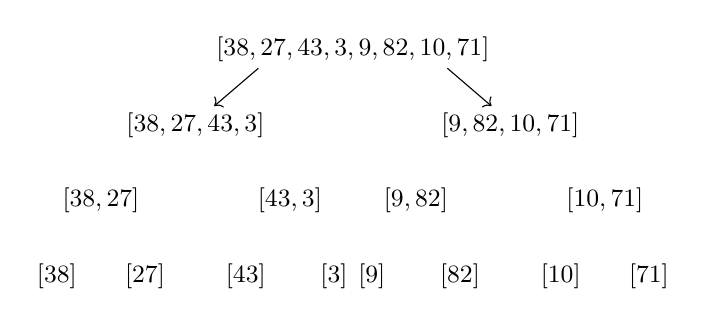
\begin{tikzpicture}[scale=0.8, every node/.style={font=\small}]
    % Level 0
    \node at (4, 0) {$[38, 27, 43, 3, 9, 82, 10, 71]$};
    
    % Level 1
    \node at (1.5, -1.2) {$[38, 27, 43, 3]$};
    \node at (6.5, -1.2) {$[9, 82, 10, 71]$};
    \draw[->] (2.5, -0.3) -- (1.8, -0.9);
    \draw[->] (5.5, -0.3) -- (6.2, -0.9);
    
    % Level 2
    \node at (0, -2.4) {$[38, 27]$};
    \node at (3, -2.4) {$[43, 3]$};
    \node at (5, -2.4) {$[9, 82]$};
    \node at (8, -2.4) {$[10, 71]$};
    
    % Level 3
    \node at (-0.7, -3.6) {$[38]$};
    \node at (0.7, -3.6) {$[27]$};
    \node at (2.3, -3.6) {$[43]$};
    \node at (3.7, -3.6) {$[3]$};
    \node at (4.3, -3.6) {$[9]$};
    \node at (5.7, -3.6) {$[82]$};
    \node at (7.3, -3.6) {$[10]$};
    \node at (8.7, -3.6) {$[71]$};
\end{tikzpicture}
\end{center}

\end{blackboard}

\begin{blackboard}[合并过程（自底向上）]

\textbf{第1轮合并}：相邻两个元素合并
\begin{itemize}
    \item $[38] + [27] \to [27, 38]$
    \item $[43] + [3] \to [3, 43]$
    \item $[9] + [82] \to [9, 82]$
    \item $[10] + [71] \to [10, 71]$
\end{itemize}

\textbf{第2轮合并}：
\begin{itemize}
    \item $[27, 38] + [3, 43] \to [3, 27, 38, 43]$
    
    合并步骤：比较27和3 $\to$ 取3；比较27和43 $\to$ 取27；比较38和43 $\to$ 取38；取43
    
    \item $[9, 82] + [10, 71] \to [9, 10, 71, 82]$
\end{itemize}

\textbf{第3轮合并}：
\begin{itemize}
    \item $[3, 27, 38, 43] + [9, 10, 71, 82] \to [3, 9, 10, 27, 38, 43, 71, 82]$
\end{itemize}

\textbf{输出}：$[3, 9, 10, 27, 38, 43, 71, 82]$

\end{blackboard}

\begin{blackboard}[Merge 操作详解]

合并 $[3, 27, 38, 43]$ 和 $[9, 10, 71, 82]$：

\begin{center}
\begin{tabular}{c|cc|c|l}
\textbf{步骤} & \textbf{左指针} & \textbf{右指针} & \textbf{输出} & \textbf{操作} \\
\hline
1 & 3 & 9 & 3 & $3 < 9$，取左，左指针右移 \\
2 & 27 & 9 & 9 & $27 > 9$，取右，右指针右移 \\
3 & 27 & 10 & 10 & $27 > 10$，取右，右指针右移 \\
4 & 27 & 71 & 27 & $27 < 71$，取左，左指针右移 \\
5 & 38 & 71 & 38 & $38 < 71$，取左，左指针右移 \\
6 & 43 & 71 & 43 & $43 < 71$，取左，左指针右移 \\
7 & -- & 71 & 71 & 左边空，取右 \\
8 & -- & 82 & 82 & 左边空，取右 \\
\end{tabular}
\end{center}

\textbf{结果}：$[3, 9, 10, 27, 38, 43, 71, 82]$

\end{blackboard}

\subsection{GPU Merge Sort 的设计}

\begin{blackboard}[GPU Merge Sort 的层级并行]

\textbf{思路}：不用递归，改用\textbf{迭代}——从小到大合并。

\textbf{算法}：
\begin{enumerate}
    \item 初始：每个元素是长度1的有序数组
    \item 第1轮：相邻两个合并成长度2的有序数组（$n/2$ 次合并，\textbf{并行}）
    \item 第2轮：相邻两个合并成长度4的有序数组（$n/4$ 次合并，\textbf{并行}）
    \item $\cdots$
    \item 第 $\log n$ 轮：两个 $n/2$ 的数组合并成完整有序数组
\end{enumerate}

\textbf{每一轮内部}：所有合并操作\textbf{完全独立}，可以并行！

\end{blackboard}

\begin{figure}[ht]
\centering
\begin{tikzpicture}[scale=0.8, every node/.style={font=\small}]
    % 初始数组
    \foreach \i/\v in {0/7, 1/3, 2/8, 3/1, 4/5, 5/2, 6/9, 7/4} {
        \node[draw, minimum width=0.8cm, minimum height=0.6cm] at (\i, 0) {\v};
    }
    \node[left] at (-1, 0) {初始:};
    
    % 第1轮
    \foreach \i/\v in {0/3, 1/7, 2/1, 3/8, 4/2, 5/5, 6/4, 7/9} {
        \node[draw, minimum width=0.8cm, minimum height=0.6cm, fill=blue!10] at (\i, -1.5) {\v};
    }
    \draw[decorate, decoration={brace, amplitude=5pt}] (1.4, -1.1) -- (-0.4, -1.1);
    \draw[decorate, decoration={brace, amplitude=5pt}] (3.4, -1.1) -- (1.6, -1.1);
    \draw[decorate, decoration={brace, amplitude=5pt}] (5.4, -1.1) -- (3.6, -1.1);
    \draw[decorate, decoration={brace, amplitude=5pt}] (7.4, -1.1) -- (5.6, -1.1);
    \node[left] at (-1, -1.5) {第1轮:};
    \node[right, gpugreen] at (8, -1.5) {4路并行};
    
    % 第2轮
    \foreach \i/\v in {0/1, 1/3, 2/7, 3/8, 4/2, 5/4, 6/5, 7/9} {
        \node[draw, minimum width=0.8cm, minimum height=0.6cm, fill=blue!20] at (\i, -3) {\v};
    }
    \draw[decorate, decoration={brace, amplitude=5pt}] (3.4, -2.6) -- (-0.4, -2.6);
    \draw[decorate, decoration={brace, amplitude=5pt}] (7.4, -2.6) -- (3.6, -2.6);
    \node[left] at (-1, -3) {第2轮:};
    \node[right, gpugreen] at (8, -3) {2路并行};
    
    % 第3轮
    \foreach \i/\v in {0/1, 1/2, 2/3, 3/4, 4/5, 5/7, 6/8, 7/9} {
        \node[draw, minimum width=0.8cm, minimum height=0.6cm, fill=blue!30] at (\i, -4.5) {\v};
    }
    \node[left] at (-1, -4.5) {第3轮:};
    \node[right, gpugreen] at (8, -4.5) {1路（串行瓶颈）};
\end{tikzpicture}
\caption{GPU Merge Sort：每轮内的合并操作并行执行}
\end{figure}

\subsection{单次合并的并行化}

\begin{blackboard}[并行合并：Merge 操作的GPU化]

\textbf{问题}：合并两个有序数组 $A[0..m-1]$ 和 $B[0..k-1]$

\textbf{串行方法}：双指针，$O(m+k)$

\textbf{并行方法}：每个输出位置独立计算！

对于输出位置 $i$，需要确定 $C[i]$ 来自 $A$ 还是 $B$。

\textbf{关键洞察}：$C[i]$ 是 $A \cup B$ 中第 $i$ 小的元素。

设 $C[i] = A[j]$，则：
\begin{itemize}
    \item $A$ 中有 $j$ 个元素 $\leq A[j]$
    \item $B$ 中有 $i - j$ 个元素 $< A[j]$（用二分查找确定）
\end{itemize}

\textbf{算法}：对每个 $i \in \{0, \ldots, m+k-1\}$：
\begin{enumerate}
    \item 二分搜索找到正确的 $(j, i-j)$ 分割
    \item 确定 $C[i]$ 的值
\end{enumerate}

\textbf{复杂度}：$O(\log(m+k))$ per thread，$(m+k)$ threads

总工作量 $O((m+k)\log(m+k))$，但并行时间 $O(\log(m+k))$！

\end{blackboard}

\begin{experiment}[GPU Merge Sort]
\begin{lstlisting}
import cupy as cp
import numpy as np
import time

def gpu_merge_sort_simple(arr):
    """简化版GPU Merge Sort：利用层级并行"""
    n = len(arr)
    d_arr = cp.asarray(arr)
    
    width = 1
    while width < n:
        # 每个block处理一对相邻的子数组
        # 这里用CuPy的argsort简化，实际应该写CUDA kernel
        for start in range(0, n, 2 * width):
            mid = min(start + width, n)
            end = min(start + 2 * width, n)
            if mid < end:
                merged = cp.concatenate([
                    d_arr[start:mid], 
                    d_arr[mid:end]
                ])
                indices = cp.argsort(merged)
                d_arr[start:end] = merged[indices]
        width *= 2
    
    return cp.asnumpy(d_arr)

# 对比测试
n = 1_000_000
arr = np.random.rand(n).astype(np.float32)

# CPU排序
start = time.time()
sorted_cpu = np.sort(arr.copy())
print(f"CPU numpy.sort: {time.time() - start:.3f}s")

# GPU排序(CuPy内置)
d_arr = cp.asarray(arr)
cp.cuda.Stream.null.synchronize()
start = time.time()
sorted_gpu = cp.sort(d_arr)
cp.cuda.Stream.null.synchronize()
print(f"GPU cupy.sort: {time.time() - start:.3f}s")
\end{lstlisting}

\textbf{典型结果}（$n = 10^6$）：
\begin{itemize}
    \item CPU \texttt{numpy.sort}: 0.08s
    \item GPU \texttt{cupy.sort}: 0.01s
    \item 加速比：$\sim 8\times$
\end{itemize}
\end{experiment}

%========================================
\section{GPU 排序的最佳选择：基数排序}
%========================================

\subsection{为什么基数排序适合GPU？}

\begin{blackboard}[比较排序 vs 非比较排序]

\textbf{比较排序}（Merge Sort, Quick Sort）：
\begin{itemize}
    \item 基于元素两两比较
    \item 下界 $\Omega(n \log n)$
    \item 依赖关系复杂，难以完全并行
\end{itemize}

\textbf{非比较排序}（Counting Sort, Radix Sort）：
\begin{itemize}
    \item 利用元素的数值特性
    \item 可以达到 $O(n)$
    \item \textbf{天然适合并行}！
\end{itemize}

\textbf{GPU排序的实际选择}：CUDA库（Thrust, CUB）默认用\textbf{基数排序}！

\end{blackboard}

\subsection{基数排序原理}

\begin{blackboard}[基数排序（Radix Sort）]

\textbf{核心思想}：从最低位到最高位，逐位排序。每位使用\textbf{稳定排序}。

\textbf{为什么要稳定？}

稳定排序保持相等元素的相对顺序。

当高位相同时，低位的顺序已经排好，稳定排序不会打乱它！

\textbf{算法}：
\begin{algorithmic}[1]
\FOR{$d = 0$ to $D-1$}
    \STATE 按第 $d$ 位对数组进行\textbf{稳定排序}（通常用计数排序）
\ENDFOR
\end{algorithmic}

\textbf{复杂度}：$O(D \cdot (n + k))$，其中 $D$ = 位数，$k$ = 每位的取值范围

对于32位整数，$D = 32$，若按8位分组则 $D = 4$，$k = 256$

\end{blackboard}

\begin{blackboard}[基数排序手算例子]

\textbf{输入}：$[329, 457, 657, 839, 436, 720, 355]$

按\textbf{十进制}每位排序（$k = 10$）：

\textbf{第1轮：按个位排序}
\begin{center}
\begin{tabular}{c|l}
个位 & 数字 \\
\hline
0 & 720 \\
5 & 355 \\
6 & 436 \\
7 & 457, 657 \\
9 & 329, 839 \\
\end{tabular}
\end{center}
结果：$[720, 355, 436, 457, 657, 329, 839]$

\textbf{第2轮：按十位排序}（保持稳定性！）
\begin{center}
\begin{tabular}{c|l}
十位 & 数字 \\
\hline
2 & 720, 329 \\
3 & 436, 839 \\
5 & 355, 457, 657 \\
\end{tabular}
\end{center}
结果：$[720, 329, 436, 839, 355, 457, 657]$

\textbf{第3轮：按百位排序}
\begin{center}
\begin{tabular}{c|l}
百位 & 数字 \\
\hline
3 & 329, 355 \\
4 & 436, 457 \\
6 & 657 \\
7 & 720 \\
8 & 839 \\
\end{tabular}
\end{center}
结果：$[329, 355, 436, 457, 657, 720, 839]$ ✓ 排序完成！

\end{blackboard}

\begin{blackboard}[稳定性的关键作用]

\textbf{观察第3轮}：329 和 355 的百位都是 3

为什么 329 在 355 前面？

因为第2轮后，329 在 355 前面（十位 2 < 5）

第3轮的稳定排序\textbf{保持了这个顺序}！

\textbf{反例}：如果第3轮用不稳定排序，可能得到 $[355, 329, \ldots]$，错误！

\end{blackboard}

\subsection{计数排序：基数排序的基础}

\begin{blackboard}[计数排序（Counting Sort）]

\textbf{问题}：排序 $n$ 个元素，每个元素的值在 $[0, k-1]$ 范围内

\textbf{算法}：
\begin{algorithmic}[1]
\STATE \COMMENT{Step 1: 计数}
\FOR{$i = 0$ to $n-1$}
    \STATE $count[A[i]] \gets count[A[i]] + 1$
\ENDFOR
\STATE
\STATE \COMMENT{Step 2: 前缀和（确定每个值的起始位置）}
\FOR{$i = 1$ to $k-1$}
    \STATE $count[i] \gets count[i] + count[i-1]$
\ENDFOR
\STATE
\STATE \COMMENT{Step 3: 放置元素（从后往前保证稳定性）}
\FOR{$i = n-1$ down to $0$}
    \STATE $count[A[i]] \gets count[A[i]] - 1$
    \STATE $output[count[A[i]]] \gets A[i]$
\ENDFOR
\end{algorithmic}

\textbf{复杂度}：$O(n + k)$

\end{blackboard}

\begin{blackboard}[计数排序手算]

\textbf{输入}：$A = [4, 2, 2, 8, 3, 3, 1]$，$k = 9$

\textbf{Step 1: 计数}
\begin{center}
\begin{tabular}{c|ccccccccc}
值 & 0 & 1 & 2 & 3 & 4 & 5 & 6 & 7 & 8 \\
\hline
count & 0 & 1 & 2 & 2 & 1 & 0 & 0 & 0 & 1 \\
\end{tabular}
\end{center}

\textbf{Step 2: 前缀和}（count[i] = 值 $\leq i$ 的元素个数）
\begin{center}
\begin{tabular}{c|ccccccccc}
值 & 0 & 1 & 2 & 3 & 4 & 5 & 6 & 7 & 8 \\
\hline
count & 0 & 1 & 3 & 5 & 6 & 6 & 6 & 6 & 7 \\
\end{tabular}
\end{center}

\textbf{Step 3: 放置}（从后往前）
\begin{itemize}
    \item $A[6]=1$: $count[1]=1 \to 0$, $output[0]=1$
    \item $A[5]=3$: $count[3]=5 \to 4$, $output[4]=3$
    \item $A[4]=3$: $count[3]=4 \to 3$, $output[3]=3$
    \item $A[3]=8$: $count[8]=7 \to 6$, $output[6]=8$
    \item $A[2]=2$: $count[2]=3 \to 2$, $output[2]=2$
    \item $A[1]=2$: $count[2]=2 \to 1$, $output[1]=2$
    \item $A[0]=4$: $count[4]=6 \to 5$, $output[5]=4$
\end{itemize}

\textbf{输出}：$[1, 2, 2, 3, 3, 4, 8]$ ✓

\end{blackboard}

\subsection{GPU 基数排序}

\begin{gpubox}[基数排序的GPU并行性]

\textbf{每一轮（按某一位排序）的三个步骤}：

\textbf{Step 1: 计数} → \textbf{完全并行}
\begin{itemize}
    \item 每个线程统计自己负责的元素
    \item 使用原子操作更新全局计数
    \item 或：先局部计数，再归约
\end{itemize}

\textbf{Step 2: 前缀和} → \textbf{高度并行}
\begin{itemize}
    \item 经典并行算法：\textbf{Blelloch scan}，$O(\log k)$ 并行时间
    \item \textbf{上扫（Upsweep / Reduce）阶段}：构建规约树，从叶向根，每层相邻元素两两相加，$\lceil \log_2 k \rceil$ 轮后根节点保存总和
    \item \textbf{下扫（Downsweep）阶段}：将根节点置零，从根向叶，每层节点将自身值传给左孩子，并将左孩子原值加上自身值后传给右孩子，$\lceil \log_2 k \rceil$ 轮后各叶节点得到前缀和
    \item 两阶段共 $O(\log k)$ 轮，每轮 $O(k)$ 次加法 $\Rightarrow$ 总工作量 $O(k \log k)$，并行时间 $O(\log k)$
\end{itemize}

\textbf{Step 3: 放置} → \textbf{完全并行}
\begin{itemize}
    \item 每个元素独立计算自己的目标位置
    \item 使用原子操作避免冲突
\end{itemize}

\textbf{总并行复杂度}：$O(D \cdot \log n)$，其中 $D$ = 轮数

\end{gpubox}

\begin{figure}[ht]
\centering
\begin{tikzpicture}[scale=0.7]
    % 输入数据
    \node[left] at (-1, 3) {\textbf{输入}:};
    \foreach \i/\v in {0/5, 1/3, 2/7, 3/1, 4/6, 5/2, 6/4, 7/0} {
        \node[draw, minimum width=0.8cm, minimum height=0.6cm] at (\i, 3) {\v};
    }
    
    % 按最低位分桶
    \node[left] at (-1, 1.5) {\textbf{按位0分桶}:};
    \draw[->] (3.5, 2.5) -- (3.5, 2);
    
    % 桶0（偶数）
    \node at (-0.5, 0.5) {桶0:};
    \foreach \i/\v in {0/0, 1/2, 2/4, 3/6} {
        \node[draw, fill=blue!20, minimum width=0.8cm, minimum height=0.6cm] at (\i+0.5, 0.5) {\v};
    }
    
    % 桶1（奇数）
    \node at (-0.5, -0.5) {桶1:};
    \foreach \i/\v in {0/1, 1/3, 2/5, 3/7} {
        \node[draw, fill=red!20, minimum width=0.8cm, minimum height=0.6cm] at (\i+0.5, -0.5) {\v};
    }
    
    % 合并
    \draw[->] (3.5, -1) -- (3.5, -1.5);
    \node[left] at (-1, -2) {\textbf{合并}:};
    \foreach \i/\v in {0/0, 1/2, 2/4, 3/6, 4/1, 5/3, 6/5, 7/7} {
        \node[draw, minimum width=0.8cm, minimum height=0.6cm] at (\i, -2) {\v};
    }
    
    % 并行标注
    \draw[decorate, decoration={brace, amplitude=5pt}] (4.5, 0.8) -- (4.5, -0.8);
    \node[right, gpugreen] at (4.7, 0) {\small 并行分桶};
\end{tikzpicture}
\caption{基数排序第一轮：按最低位分成偶数桶和奇数桶}
\end{figure}

\begin{blackboard}[GPU 基数排序的优化技巧]

\textbf{1. 按多位分组}
\begin{itemize}
    \item 不按1位，而按4位或8位分组
    \item 减少轮数：32位整数只需 4 轮（8位/轮）
    \item 桶数增加：$2^8 = 256$ 个桶
\end{itemize}

\textbf{2. 局部排序 + 全局合并}
\begin{itemize}
    \item 每个线程块先对局部数据排序
    \item 再合并各块的结果
    \item 减少全局内存访问
\end{itemize}

\textbf{3. 避免原子操作冲突}
\begin{itemize}
    \item 使用线程块级别的共享内存计数
    \item 块内归约后再更新全局计数
\end{itemize}

\end{blackboard}

\begin{complexitybox}[排序算法GPU性能对比]

\begin{center}
\begin{tabular}{l|ccc}
\textbf{算法} & \textbf{串行复杂度} & \textbf{并行复杂度} & \textbf{GPU适合度} \\
\hline
Merge Sort & $O(n \log n)$ & $O(\log^2 n)$ & ⭐⭐ \\
Quick Sort & $O(n \log n)$ & $O(\log^2 n)$ 期望 & ⭐ \\
Bitonic Sort & $O(n \log^2 n)$ & $O(\log^2 n)$ & ⭐⭐⭐ \\
\textbf{Radix Sort} & $O(Dn)$ & $O(D \log n)$ & ⭐⭐⭐⭐ \\
\end{tabular}
\end{center}

\textbf{实际性能}（NVIDIA GPU，$n = 10^8$ 个32位整数）：
\begin{itemize}
    \item Thrust radix sort: $\sim 50$ ms
    \item Thrust merge sort: $\sim 200$ ms
    \item CPU std::sort: $\sim 8000$ ms
\end{itemize}

基数排序比并行归并排序快 $4\times$，比CPU快 $160\times$！

\end{complexitybox}

%========================================
\section{分治的GPU化：FFT}
%========================================

\subsection{FFT的蝴蝶操作}

\begin{blackboard}[Cooley-Tukey FFT 回顾]

\textbf{DFT 定义}：给定 $x_0, \ldots, x_{n-1}$，计算
\[
X_k = \sum_{j=0}^{n-1} x_j \cdot e^{-2\pi i jk/n}, \quad k = 0, \ldots, n-1
\]

直接计算：$O(n^2)$

\textbf{FFT 的分治思想}：将 DFT 分解为奇偶两部分

设 $\omega_n = e^{-2\pi i/n}$，则：
\begin{align*}
X_k &= \sum_{j=0}^{n/2-1} x_{2j} \omega_n^{2jk} + \sum_{j=0}^{n/2-1} x_{2j+1} \omega_n^{(2j+1)k} \\
&= \underbrace{\sum_{j=0}^{n/2-1} x_{2j} \omega_{n/2}^{jk}}_{E_k} + \omega_n^k \underbrace{\sum_{j=0}^{n/2-1} x_{2j+1} \omega_{n/2}^{jk}}_{O_k}
\end{align*}

其中 $E_k$ 是偶数项的 $n/2$ 点 DFT，$O_k$ 是奇数项的 $n/2$ 点 DFT。

\textbf{蝴蝶操作}：
\[
X_k = E_k + \omega_n^k O_k, \quad X_{k+n/2} = E_k - \omega_n^k O_k
\]

\end{blackboard}

\begin{figure}[ht]
\centering
\begin{tikzpicture}[x=1.8cm,y=0.8cm,>=stealth]

    % 标题
    \node[font=\small\bfseries] at (1.8,1.4) {8点 radix-2 DIT FFT 的蝴蝶结构};

    %--------------------------------
    % 输入与输出节点
    %--------------------------------
    \foreach \i/\lab in {
        0/{x_0},1/{x_4},2/{x_2},3/{x_6},
        4/{x_1},5/{x_5},6/{x_3},7/{x_7}}{
        \fill (0,-\i) circle (1.5pt);
        \node[left] at (0,-\i) {$\lab$};
    }

    \foreach \i in {0,...,7}{
        \fill (4,-\i) circle (1.5pt);
        \node[right] at (4,-\i) {$X_{\i}$};
    }

    %--------------------------------
    % Stage labels
    %--------------------------------
    \node[above] at (1,0.2) {Stage 1};
    \node[above] at (2,0.2) {Stage 2};
    \node[above] at (3,0.2) {Stage 3};

    %--------------------------------
    % 中间节点
    %--------------------------------
    \foreach \x in {1,2,3}{
        \foreach \i in {0,...,7}{
            \fill (\x,-\i) circle (1.2pt);
        }
    }

    %--------------------------------
    % Stage 1: 相邻配对
    % pairs: (0,1), (2,3), (4,5), (6,7)
    %--------------------------------
    \foreach \a/\b in {0/1,2/3,4/5,6/7}{
        \draw[->] (0,-\a) -- (1,-\a);
        \draw[->] (0,-\b) -- (1,-\a);
        \draw[->] (0,-\a) -- (1,-\b);
        \draw[->] (0,-\b) -- (1,-\b);

        % 可选：竖虚线强调一个butterfly
        \draw[dashed,gray!60] (0.5,-\a) -- (0.5,-\b);
    }


    %--------------------------------
    % Stage 2: 跨2配对
    % pairs: (0,2), (1,3), (4,6), (5,7)
    %--------------------------------
    \foreach \a/\b in {0/2,1/3,4/6,5/7}{
        \draw[->] (1,-\a) -- (2,-\a);
        \draw[->] (1,-\b) -- (2,-\a);
        \draw[->] (1,-\a) -- (2,-\b);
        \draw[->] (1,-\b) -- (2,-\b);

        \draw[dashed,gray!60] (1.5,-\a) -- (1.5,-\b);
    }

    %--------------------------------
    % Stage 3: 跨4配对
    % pairs: (0,4), (1,5), (2,6), (3,7)
    %--------------------------------
    \foreach \a/\b in {0/4,1/5,2/6,3/7}{
        \draw[->] (2,-\a) -- (3,-\a);
        \draw[->] (2,-\b) -- (3,-\a);
        \draw[->] (2,-\a) -- (3,-\b);
        \draw[->] (2,-\b) -- (3,-\b);

        \draw[dashed,gray!60] (2.5,-\a) -- (2.5,-\b);
    }



    %--------------------------------
    % 输出连线
    %--------------------------------
    \foreach \i in {0,...,7}{
        \draw[->] (3,-\i) -- (4,-\i);
    }

    %--------------------------------
    % 左右说明
    %--------------------------------
    \node[align=center, font=\scriptsize] at (0,-9.8)
    {输入按 bit-reversal 顺序排列\\$\{x_0,x_4,x_2,x_6,x_1,x_5,x_3,x_7\}$};

    \node[align=center, font=\scriptsize] at (4,-9.8)
    {输出为自然顺序\\$\{X_0,\dots,X_7\}$};

\end{tikzpicture}
\caption{8点 radix-2 DIT FFT 的蝴蝶结构示意图。每个 stage 内的 butterfly 单元彼此独立，因此可并行执行；但不同 stage 之间存在顺序依赖。图中输入采用 bit-reversal 顺序，因此输出为自然顺序。}
\label{fig:fft_butterfly_8point}
\end{figure}

\begin{blackboard}[4点 FFT 数值例子]

\textbf{输入}：$x = [1, 2, 3, 4]$

\textbf{目标}：计算 DFT $X_k = \sum_{j=0}^{3} x_j \cdot e^{-2\pi i jk/4}$

\textbf{旋转因子}：$\omega_4 = e^{-2\pi i/4} = e^{-\pi i/2} = -i$

所以：$\omega_4^0 = 1$，$\omega_4^1 = -i$，$\omega_4^2 = -1$，$\omega_4^3 = i$

\textbf{Bit-reversal 排列}：
\begin{center}
\begin{tabular}{c|c|c}
原索引 & 二进制 & 反转后 \\
\hline
0 & 00 & 00 $\to$ 0 \\
1 & 01 & 10 $\to$ 2 \\
2 & 10 & 01 $\to$ 1 \\
3 & 11 & 11 $\to$ 3 \\
\end{tabular}
\end{center}

重排后：$[x_0, x_2, x_1, x_3] = [1, 3, 2, 4]$

\textbf{Stage 1}：2点 DFT（两组）
\begin{itemize}
    \item 蝴蝶1：$[1, 3] \to [1+3, 1-3] = [4, -2]$
    \item 蝴蝶2：$[2, 4] \to [2+4, 2-4] = [6, -2]$
\end{itemize}
结果：$[4, -2, 6, -2]$

\textbf{Stage 2}：4点 DFT
\begin{itemize}
    \item $X_0 = 4 + \omega_4^0 \cdot 6 = 4 + 6 = 10$
    \item $X_1 = -2 + \omega_4^1 \cdot (-2) = -2 + (-i)(-2) = -2 + 2i$
    \item $X_2 = 4 + \omega_4^2 \cdot 6 = 4 - 6 = -2$
    \item $X_3 = -2 + \omega_4^3 \cdot (-2) = -2 + i(-2) = -2 - 2i$
\end{itemize}

\textbf{输出}：$X = [10, -2+2i, -2, -2-2i]$

\textbf{验证}：$X_0 = 1+2+3+4 = 10$ ✓（直流分量 = 求和）

\end{blackboard}

\begin{gpubox}[FFT 的 GPU 并行性]

\textbf{结构}：$\log_2 n$ 个 stages，每个 stage 有 $n/2$ 个蝴蝶操作。

\textbf{并行性}：
\begin{itemize}
    \item 同一 stage 内：所有蝴蝶操作\textbf{完全独立}
    \item 不同 stage：必须\textbf{顺序}执行（后一个依赖前一个）
\end{itemize}

\textbf{GPU 实现要点}：
\begin{itemize}
    \item 每个线程处理一个蝴蝶操作
    \item Stage 之间用 \texttt{\_\_syncthreads()} 同步
    \item 利用 shared memory 减少 global memory 访问
\end{itemize}

\textbf{复杂度}：
\begin{itemize}
    \item 串行：$O(n \log n)$
    \item 并行（$n/2$ 个处理器）：$O(\log n)$
\end{itemize}

\end{gpubox}

%========================================
\section{动态规划}
%========================================

\subsection{DP 的核心思想}

\begin{blackboard}[动态规划的两个关键性质]

\textbf{性质1：最优子结构}

问题的最优解\textbf{包含}子问题的最优解。

例：最短路径——$s \to t$ 的最短路径经过 $v$，则 $s \to v$ 部分也是最短路径。

\textbf{性质2：重叠子问题}

不同的递归分支会求解\textbf{相同}的子问题。

例：Fibonacci $F(n) = F(n-1) + F(n-2)$，朴素递归重复计算 $F(k)$ 指数次。

\textbf{DP 的做法}：
\begin{enumerate}
    \item 定义状态（子问题的参数化）
    \item 写出状态转移方程（如何从子问题构造原问题）
    \item 确定计算顺序（保证子问题先于原问题求解）
    \item 用表格存储结果，避免重复计算
\end{enumerate}

\end{blackboard}

\subsection{证明最优子结构：剪切-粘贴法}

\begin{blackboard}[最短路径的最优子结构证明]

\textbf{命题}：设 $p = v_0 \to v_1 \to \cdots \to v_k$ 是从 $v_0$ 到 $v_k$ 的最短路径。则对任意 $0 \leq i < j \leq k$，子路径 $p_{ij} = v_i \to v_{i+1} \to \cdots \to v_j$ 是从 $v_i$ 到 $v_j$ 的最短路径。

\textbf{证明}（剪切-粘贴法/反证法）：

假设 $p_{ij}$ 不是 $v_i$ 到 $v_j$ 的最短路径。

则存在更短的路径 $p'_{ij}$，满足 $w(p'_{ij}) < w(p_{ij})$。

\textbf{剪切}：从 $p$ 中移除 $p_{ij}$

\textbf{粘贴}：用 $p'_{ij}$ 替换

得到新路径 $p' = v_0 \to \cdots \to v_i \xrightarrow{p'_{ij}} v_j \to \cdots \to v_k$

则 $w(p') = w(p) - w(p_{ij}) + w(p'_{ij}) < w(p)$

这与 $p$ 是最短路径矛盾！

\textbf{结论}：$p_{ij}$ 必须是 $v_i$ 到 $v_j$ 的最短路径。 $\square$

\end{blackboard}

\begin{insight}[剪切-粘贴法的通用模式]

\textbf{目标}：证明最优解包含子问题的最优解

\textbf{步骤}：
\begin{enumerate}
    \item 假设最优解中的某个子问题解不是最优的
    \item 用那个子问题的真正最优解"替换"它
    \item 证明替换后得到更好的解
    \item 与原解是最优矛盾
\end{enumerate}

这个方法几乎适用于所有 DP 问题的最优子结构证明。
\end{insight}

\subsection{例：编辑距离}

\begin{blackboard}[编辑距离（Levenshtein Distance）]

\textbf{问题}：给定两个字符串 $A[1..m]$ 和 $B[1..n]$，求将 $A$ 变成 $B$ 的最少操作数。

允许的操作：插入、删除、替换（各计1次）。

\textbf{状态定义}：$dp[i][j]$ = 将 $A[1..i]$ 变成 $B[1..j]$ 的最少操作数

\textbf{状态转移}：
\[
dp[i][j] = \min \begin{cases}
dp[i-1][j] + 1 & \text{（删除 $A[i]$）} \\
dp[i][j-1] + 1 & \text{（插入 $B[j]$）} \\
dp[i-1][j-1] + \mathbf{1}_{A[i] \neq B[j]} & \text{（匹配或替换）}
\end{cases}
\]

\textbf{边界条件}：
\begin{itemize}
    \item $dp[0][j] = j$（空串变成 $B[1..j]$ 需要 $j$ 次插入）
    \item $dp[i][0] = i$（$A[1..i]$ 变成空串需要 $i$ 次删除）
\end{itemize}

\textbf{计算顺序}：从左到右、从上到下填表

\textbf{时间复杂度}：$O(mn)$，空间复杂度：$O(mn)$（可优化到 $O(\min(m,n))$）

\end{blackboard}

\begin{blackboard}[编辑距离具体例子：手算填表]

\textbf{输入}：$A$ = "CAT"，$B$ = "CAR"

将 "CAT" 变成 "CAR" 需要多少次操作？

\textbf{填表过程}：

\begin{center}
\begin{tabular}{c|cccc}
$dp[i][j]$ & $\epsilon$ & C & A & R \\
\hline
$\epsilon$ & 0 & 1 & 2 & 3 \\
C & 1 & 0 & 1 & 2 \\
A & 2 & 1 & 0 & 1 \\
T & 3 & 2 & 1 & \textcolor{red}{1} \\
\end{tabular}
\end{center}

\textbf{逐格计算}：

$dp[1][1]$ ($A[1]$=C, $B[1]$=C)：字符相同！
\[
dp[1][1] = \min(dp[0][1]+1, dp[1][0]+1, dp[0][0]+0) = \min(2, 2, 0) = 0
\]

$dp[1][2]$ ($A[1]$=C, $B[2]$=A)：字符不同
\[
dp[1][2] = \min(dp[0][2]+1, dp[1][1]+1, dp[0][1]+1) = \min(3, 1, 2) = 1
\]

$dp[2][2]$ ($A[2]$=A, $B[2]$=A)：字符相同！
\[
dp[2][2] = \min(dp[1][2]+1, dp[2][1]+1, dp[1][1]+0) = \min(2, 2, 0) = 0
\]

$dp[3][3]$ ($A[3]$=T, $B[3]$=R)：字符不同
\[
dp[3][3] = \min(dp[2][3]+1, dp[3][2]+1, dp[2][2]+1) = \min(2, 2, 1) = 1
\]

\textbf{答案}：$dp[3][3] = 1$（把 T 替换成 R）

\end{blackboard}

\begin{blackboard}[编辑距离状态转移的证明]

\textbf{命题}：状态转移方程正确，即
\[
dp[i][j] = \min \begin{cases}
dp[i-1][j] + 1 \\
dp[i][j-1] + 1 \\
dp[i-1][j-1] + \mathbf{1}_{A[i] \neq B[j]}
\end{cases}
\]

\textbf{证明}：

设 $S$ 是将 $A[1..i]$ 变成 $B[1..j]$ 的任意最优操作序列。

考虑 $S$ 的\textbf{最后一步操作}对 $A[i]$ 做了什么：

\textbf{Case 1}：最后删除了 $A[i]$

则 $S$ 的前面部分将 $A[1..i-1]$ 变成 $B[1..j]$

$\Rightarrow$ $|S| = dp[i-1][j] + 1$

（如果前面部分不是最优，可以剪切-粘贴得到矛盾）

\textbf{Case 2}：最后插入了 $B[j]$

则 $S$ 的前面部分将 $A[1..i]$ 变成 $B[1..j-1]$

$\Rightarrow$ $|S| = dp[i][j-1] + 1$

\textbf{Case 3}：$A[i]$ 和 $B[j]$ 匹配（或被替换）

则 $S$ 的前面部分将 $A[1..i-1]$ 变成 $B[1..j-1]$

$\Rightarrow$ $|S| = dp[i-1][j-1] + \mathbf{1}_{A[i] \neq B[j]}$

\textbf{结论}：最优解必落入三种情况之一，取最小值即可。 $\square$

\end{blackboard}

\begin{figure}[ht]
\centering
\begin{tikzpicture}[scale=0.7]
    % DP表格
    \node at (-1, 5) {};
    \node at (0, 5) {$\epsilon$};
    \node at (1, 5) {k};
    \node at (2, 5) {i};
    \node at (3, 5) {t};
    \node at (4, 5) {t};
    \node at (5, 5) {e};
    \node at (6, 5) {n};
    
    \node at (-1, 4) {$\epsilon$};
    \node at (-1, 3) {s};
    \node at (-1, 2) {i};
    \node at (-1, 1) {t};
    \node at (-1, 0) {t};
    \node at (-1, -1) {i};
    \node at (-1, -2) {n};
    \node at (-1, -3) {g};
    
    % 填入数值
    \foreach \j in {0,...,6} {
        \node at (\j, 4) {\j};
    }
    \foreach \i in {0,...,7} {
        \node at (0, 4-\i) {\i};
    }
    
    % 部分DP值
    \node at (1, 3) {1};
    \node at (2, 3) {2};
    \node at (1, 2) {2};
    \node[red] at (2, 2) {1};
    \node at (3, 2) {2};
    \node at (2, 1) {2};
    \node at (3, 1) {1};
    \node[red] at (4, 1) {1};
    
    % 依赖箭头
    \draw[->, thick, blue] (1.3, 2.3) -- (1.7, 1.7);
    \draw[->, thick, blue] (2.3, 1.3) -- (2.7, 0.7);
    
    % 对角线标注
    \draw[dashed, orange, thick] (-0.5, 4.5) -- (6.5, -2.5);
    \node[orange, right] at (7, 1) {对角线方向};
\end{tikzpicture}
\caption{编辑距离 DP 表格：每个格子依赖左、上、左上三个格子}
\end{figure}

\subsection{例：最长公共子序列 (LCS)}

\begin{blackboard}[LCS 问题定义]

\textbf{问题}：给定两个序列 $X = x_1 x_2 \cdots x_m$ 和 $Y = y_1 y_2 \cdots y_n$，求最长公共子序列的长度。

\textbf{子序列}：从原序列中删除若干元素（可以不连续）得到的序列。

\textbf{例}：$X = \text{ABCBDAB}$，$Y = \text{BDCABA}$

LCS = BCBA 或 BDAB，长度 = 4

\textbf{状态定义}：$dp[i][j]$ = $X[1..i]$ 和 $Y[1..j]$ 的 LCS 长度

\end{blackboard}

\begin{blackboard}[LCS 最优子结构的证明]

\textbf{命题}：设 $Z = z_1 z_2 \cdots z_k$ 是 $X[1..m]$ 和 $Y[1..n]$ 的一个 LCS。

\begin{enumerate}
    \item 若 $x_m = y_n$，则 $z_k = x_m = y_n$，且 $Z[1..k-1]$ 是 $X[1..m-1]$ 和 $Y[1..n-1]$ 的 LCS
    \item 若 $x_m \neq y_n$ 且 $z_k \neq x_m$，则 $Z$ 是 $X[1..m-1]$ 和 $Y[1..n]$ 的 LCS
    \item 若 $x_m \neq y_n$ 且 $z_k \neq y_n$，则 $Z$ 是 $X[1..m]$ 和 $Y[1..n-1]$ 的 LCS
\end{enumerate}

\textbf{证明（情况1）}：

假设 $x_m = y_n$。

\textbf{Step 1}：证明 $z_k = x_m = y_n$

反证：若 $z_k \neq x_m$，则可以将 $x_m$ 附加到 $Z$ 末尾，得到更长的公共子序列，矛盾。

\textbf{Step 2}：证明 $Z[1..k-1]$ 是 $X[1..m-1]$ 和 $Y[1..n-1]$ 的 LCS

显然 $Z[1..k-1]$ 是 $X[1..m-1]$ 和 $Y[1..n-1]$ 的公共子序列。

若存在更长的公共子序列 $W$，长度 $> k-1$，则 $W$ 后接 $x_m$ 是 $X$ 和 $Y$ 的公共子序列，长度 $> k$，与 $Z$ 是 LCS 矛盾。 $\square$

\end{blackboard}

\begin{blackboard}[LCS 状态转移方程]

由最优子结构，状态转移方程为：

\[
dp[i][j] = \begin{cases}
0 & \text{if } i = 0 \text{ or } j = 0 \\
dp[i-1][j-1] + 1 & \text{if } x_i = y_j \\
\max(dp[i-1][j], dp[i][j-1]) & \text{if } x_i \neq y_j
\end{cases}
\]

\textbf{正确性证明}（归纳法）：

\textbf{归纳假设}：对所有 $i' < i$ 或 $j' < j$，$dp[i'][j']$ 正确。

\textbf{归纳步骤}：

\textbf{Case} $x_i = y_j$：

由情况1，LCS 以 $x_i = y_j$ 结尾，去掉后是 $X[1..i-1]$ 和 $Y[1..j-1]$ 的 LCS。

由归纳假设，$dp[i-1][j-1]$ 正确，故 $dp[i][j] = dp[i-1][j-1] + 1$。

\textbf{Case} $x_i \neq y_j$：

LCS 要么不包含 $x_i$（情况2），要么不包含 $y_j$（情况3）。

由归纳假设，$dp[i-1][j]$ 和 $dp[i][j-1]$ 正确，取最大值即可。 $\square$

\end{blackboard}

\begin{blackboard}[LCS 具体例子：手算填表]

\textbf{输入}：$X = \text{ABCBDAB}$（长度7），$Y = \text{BDCABA}$（长度6）

\textbf{填表过程}（展示关键步骤）：

\textbf{初始化}：第0行和第0列全为0

\textbf{填 $dp[1][*]$}（$X[1] = A$）：
\begin{itemize}
    \item $dp[1][1]$：$A \neq B$，$\max(dp[0][1], dp[1][0]) = \max(0, 0) = 0$
    \item $dp[1][2]$：$A \neq D$，$\max(dp[0][2], dp[1][1]) = \max(0, 0) = 0$
    \item $dp[1][3]$：$A \neq C$，$\max(dp[0][3], dp[1][2]) = \max(0, 0) = 0$
    \item $dp[1][4]$：$A = A$（$Y[4]=A$），$dp[0][3] + 1 = 0 + 1 = 1$
    \item $dp[1][5]$：$A \neq B$（$Y[5]=B$），$\max(dp[0][5], dp[1][4]) = \max(0, 1) = 1$
    \item $dp[1][6]$：$A = A$（$Y[6]=A$），$dp[0][5] + 1 = 0 + 1 = 1$
\end{itemize}

\textbf{填 $dp[2][*]$}（$X[2] = B$）：
\begin{itemize}
    \item $dp[2][1]$：$B = B$（$Y[1]=B$），$dp[1][0] + 1 = 0 + 1 = 1$
    \item $dp[2][2]$：$B \neq D$，$\max(dp[1][2], dp[2][1]) = \max(0, 1) = 1$
    \item $dp[2][3]$：$B \neq C$，$\max(dp[1][3], dp[2][2]) = \max(0, 1) = 1$
    \item $dp[2][4]$：$B \neq A$，$\max(dp[1][4], dp[2][3]) = \max(1, 1) = 1$
    \item $dp[2][5]$：$B = B$（$Y[5]=B$），$dp[1][4] + 1 = 1 + 1 = 2$
    \item $dp[2][6]$：$B \neq A$，$\max(dp[1][6], dp[2][5]) = \max(1, 2) = 2$
\end{itemize}

\end{blackboard}

\begin{figure}[ht]
\centering
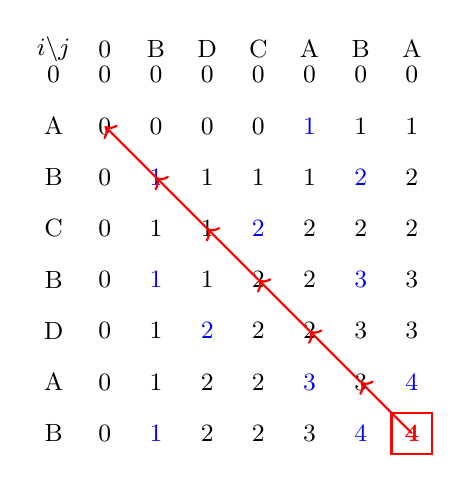
\begin{tikzpicture}[scale=0.65]
    % 表头
    \node at (-1, 0.5) {\small $i \backslash j$};
    \node at (0, 0.5) {\small 0};
    \foreach \j/\c in {1/B, 2/D, 3/C, 4/A, 5/B, 6/A} {
        \node at (\j, 0.5) {\small \c};
    }
    
    % 行标签
    \node at (-1, 0) {\small 0};
    \foreach \i/\c in {1/A, 2/B, 3/C, 4/B, 5/D, 6/A, 7/B} {
        \node at (-1, -\i) {\small \c};
    }
    
    % 填入DP值
    % i=0
    \foreach \j in {0,...,6} {
        \node at (\j, 0) {\small 0};
    }
    
    % i=1 (A)
    \node at (0, -1) {\small 0};
    \node at (1, -1) {\small 0};
    \node at (2, -1) {\small 0};
    \node at (3, -1) {\small 0};
    \node[blue] at (4, -1) {\small 1};
    \node at (5, -1) {\small 1};
    \node at (6, -1) {\small 1};
    
    % i=2 (B)
    \node at (0, -2) {\small 0};
    \node[blue] at (1, -2) {\small 1};
    \node at (2, -2) {\small 1};
    \node at (3, -2) {\small 1};
    \node at (4, -2) {\small 1};
    \node[blue] at (5, -2) {\small 2};
    \node at (6, -2) {\small 2};
    
    % i=3 (C)
    \node at (0, -3) {\small 0};
    \node at (1, -3) {\small 1};
    \node at (2, -3) {\small 1};
    \node[blue] at (3, -3) {\small 2};
    \node at (4, -3) {\small 2};
    \node at (5, -3) {\small 2};
    \node at (6, -3) {\small 2};
    
    % i=4 (B)
    \node at (0, -4) {\small 0};
    \node[blue] at (1, -4) {\small 1};
    \node at (2, -4) {\small 1};
    \node at (3, -4) {\small 2};
    \node at (4, -4) {\small 2};
    \node[blue] at (5, -4) {\small 3};
    \node at (6, -4) {\small 3};
    
    % i=5 (D)
    \node at (0, -5) {\small 0};
    \node at (1, -5) {\small 1};
    \node[blue] at (2, -5) {\small 2};
    \node at (3, -5) {\small 2};
    \node at (4, -5) {\small 2};
    \node at (5, -5) {\small 3};
    \node at (6, -5) {\small 3};
    
    % i=6 (A)
    \node at (0, -6) {\small 0};
    \node at (1, -6) {\small 1};
    \node at (2, -6) {\small 2};
    \node at (3, -6) {\small 2};
    \node[blue] at (4, -6) {\small 3};
    \node at (5, -6) {\small 3};
    \node[blue] at (6, -6) {\small 4};
    
    % i=7 (B)
    \node at (0, -7) {\small 0};
    \node[blue] at (1, -7) {\small 1};
    \node at (2, -7) {\small 2};
    \node at (3, -7) {\small 2};
    \node at (4, -7) {\small 3};
    \node[blue] at (5, -7) {\small 4};
    \node[red, font=\bfseries] at (6, -7) {\small 4};
    
    % 回溯路径
    \draw[->, thick, red] (6, -7) -- (5, -6);
    \draw[->, thick, red] (5, -6) -- (4, -5);
    \draw[->, thick, red] (4, -5) -- (3, -4);
    \draw[->, thick, red] (3, -4) -- (2, -3);
    \draw[->, thick, red] (2, -3) -- (1, -2);
    \draw[->, thick, red] (1, -2) -- (0, -1);
    
    % 答案
    \draw[thick, red] (5.6, -7.4) rectangle (6.4, -6.6);
\end{tikzpicture}
\caption{LCS 表格：$dp[7][6] = 4$。回溯路径给出 LCS = BCBA（或 BDAB）}
\end{figure}

\begin{blackboard}[LCS 回溯找具体序列]

从 $dp[m][n]$ 开始回溯：

\begin{algorithmic}[1]
\STATE $i \gets m$, $j \gets n$, $result \gets$ 空串
\WHILE{$i > 0$ and $j > 0$}
    \IF{$X[i] = Y[j]$}
        \STATE $result \gets X[i] + result$（前置）
        \STATE $i \gets i - 1$, $j \gets j - 1$
    \ELSIF{$dp[i-1][j] > dp[i][j-1]$}
        \STATE $i \gets i - 1$
    \ELSE
        \STATE $j \gets j - 1$
    \ENDIF
\ENDWHILE
\RETURN $result$
\end{algorithmic}

\textbf{例子中的回溯}：
\begin{itemize}
    \item $(7,6)$：$X[7]=B \neq Y[6]=A$，$dp[6][6]=4 > dp[7][5]=4$？否，$j \gets 5$
    \item $(7,5)$：$X[7]=B = Y[5]=B$，输出 B，$(6,4)$
    \item $(6,4)$：$X[6]=A = Y[4]=A$，输出 A，$(5,3)$
    \item $(5,3)$：$X[5]=D \neq Y[3]=C$，$dp[4][3]=2 = dp[5][2]=2$，$j \gets 2$
    \item $(5,2)$：$X[5]=D = Y[2]=D$，输出 D，$(4,1)$
    \item $(4,1)$：$X[4]=B = Y[1]=B$，输出 B，$(3,0)$
    \item 结束
\end{itemize}

\textbf{结果}：LCS = BDAB（从后往前：B, A, D, B）

\end{blackboard}

\subsection{例：0-1 背包问题}

\begin{blackboard}[0-1 背包问题]

\textbf{问题}：$n$ 个物品，第 $i$ 个重量 $w_i$，价值 $v_i$。背包容量 $W$。选择物品使总价值最大，且总重量 $\leq W$。

\textbf{状态定义}：$dp[i][j]$ = 前 $i$ 个物品、容量为 $j$ 时的最大价值

\textbf{状态转移}：
\[
dp[i][j] = \begin{cases}
dp[i-1][j] & \text{if } w_i > j \text{（放不下）} \\
\max(dp[i-1][j], dp[i-1][j-w_i] + v_i) & \text{otherwise}
\end{cases}
\]

\textbf{解释}：
\begin{itemize}
    \item $dp[i-1][j]$：不选第 $i$ 个物品
    \item $dp[i-1][j-w_i] + v_i$：选第 $i$ 个物品（前提是放得下）
\end{itemize}

\end{blackboard}

\begin{blackboard}[0-1 背包的完整算法]

\textbf{输入}：物品重量 $w[1..n]$，价值 $v[1..n]$，背包容量 $W$

\textbf{输出}：最大价值

\begin{algorithmic}[1]
\STATE \textbf{初始化}：$dp[0][j] \gets 0$ for all $j = 0, 1, \ldots, W$
\FOR{$i = 1$ to $n$}
    \FOR{$j = 0$ to $W$}
        \IF{$w[i] > j$}
            \STATE $dp[i][j] \gets dp[i-1][j]$ \COMMENT{放不下，不选}
        \ELSE
            \STATE $dp[i][j] \gets \max(dp[i-1][j], dp[i-1][j-w[i]] + v[i])$
        \ENDIF
    \ENDFOR
\ENDFOR
\RETURN $dp[n][W]$
\end{algorithmic}

\textbf{时间复杂度}：$O(nW)$（伪多项式时间）

\textbf{空间复杂度}：$O(nW)$，可优化到 $O(W)$

\end{blackboard}

\begin{blackboard}[具体例子：手算填表]

\textbf{输入}：4个物品，背包容量 $W = 5$

\begin{center}
\begin{tabular}{c|cccc}
物品 $i$ & 1 & 2 & 3 & 4 \\
\hline
重量 $w_i$ & 2 & 1 & 3 & 2 \\
价值 $v_i$ & 3 & 2 & 4 & 3 \\
\end{tabular}
\end{center}

\textbf{填表过程}：

\textbf{初始化}：$dp[0][j] = 0$（没有物品可选）

\textbf{$i = 1$}（物品1：重量2，价值3）：
\begin{itemize}
    \item $j = 0, 1$：放不下，$dp[1][j] = dp[0][j] = 0$
    \item $j = 2, 3, 4, 5$：$dp[1][j] = \max(0, dp[0][j-2] + 3) = 3$
\end{itemize}

\textbf{$i = 2$}（物品2：重量1，价值2）：
\begin{itemize}
    \item $j = 0$：放不下，$dp[2][0] = 0$
    \item $j = 1$：$dp[2][1] = \max(dp[1][1], dp[1][0] + 2) = \max(0, 2) = 2$
    \item $j = 2$：$dp[2][2] = \max(dp[1][2], dp[1][1] + 2) = \max(3, 2) = 3$
    \item $j = 3$：$dp[2][3] = \max(dp[1][3], dp[1][2] + 2) = \max(3, 5) = 5$
    \item $j = 4$：$dp[2][4] = \max(dp[1][4], dp[1][3] + 2) = \max(3, 5) = 5$
    \item $j = 5$：$dp[2][5] = \max(dp[1][5], dp[1][4] + 2) = \max(3, 5) = 5$
\end{itemize}

\end{blackboard}

\begin{figure}[ht]
\centering
\begin{tikzpicture}[scale=0.75]
    % 表头
    \node at (-1.5, 0.5) {\small $i \backslash j$};
    \foreach \j in {0,...,5} {
        \node at (\j, 0.5) {\small \j};
    }
    
    % 行标签
    \node at (-1.5, 0) {\small 0};
    \node at (-1.5, -1) {\small 1};
    \node at (-1.5, -2) {\small 2};
    \node at (-1.5, -3) {\small 3};
    \node at (-1.5, -4) {\small 4};
    
    % 物品信息
    \node[right] at (6.5, 0) {\small (无物品)};
    \node[right] at (6.5, -1) {\small $w_1=2, v_1=3$};
    \node[right] at (6.5, -2) {\small $w_2=1, v_2=2$};
    \node[right] at (6.5, -3) {\small $w_3=3, v_3=4$};
    \node[right] at (6.5, -4) {\small $w_4=2, v_4=3$};
    
    % i=0 行
    \foreach \j in {0,...,5} {
        \node at (\j, 0) {0};
    }
    
    % i=1 行
    \node at (0, -1) {0};
    \node at (1, -1) {0};
    \node[blue] at (2, -1) {3};
    \node[blue] at (3, -1) {3};
    \node[blue] at (4, -1) {3};
    \node[blue] at (5, -1) {3};
    
    % i=2 行
    \node at (0, -2) {0};
    \node[blue] at (1, -2) {2};
    \node at (2, -2) {3};
    \node[red] at (3, -2) {5};
    \node[red] at (4, -2) {5};
    \node[red] at (5, -2) {5};
    
    % i=3 行
    \node at (0, -3) {0};
    \node at (1, -3) {2};
    \node at (2, -3) {3};
    \node at (3, -3) {5};
    \node[red] at (4, -3) {6};
    \node[red] at (5, -3) {7};
    
    % i=4 行
    \node at (0, -4) {0};
    \node at (1, -4) {2};
    \node at (2, -4) {3};
    \node at (3, -4) {5};
    \node at (4, -4) {6};
    \node[red, font=\bfseries] at (5, -4) {8};
    
    % 箭头展示依赖
    \draw[->, thick, orange] (2.7, -0.8) -- (4.3, -2.2);
    \node[orange, font=\tiny] at (4.5, -1.2) {选物品2};
    
    \draw[->, thick, gray] (4, -2.8) -- (4, -3.2);
    \node[gray, font=\tiny, right] at (4.1, -3) {不选};
    
    % 最终答案
    \draw[thick, red] (4.6, -4.4) rectangle (5.4, -3.6);
    \node[red, right] at (5.5, -4) {\small 答案};
\end{tikzpicture}
\caption{0-1背包 DP 表格：$dp[4][5] = 8$，选物品 1, 2, 4（重量 $2+1+2=5$，价值 $3+2+3=8$）}
\end{figure}

\begin{blackboard}[回溯：找出选了哪些物品]

填完表后，从 $dp[n][W]$ 往回追溯：

\begin{algorithmic}[1]
\STATE $j \gets W$
\FOR{$i = n$ down to $1$}
    \IF{$dp[i][j] \neq dp[i-1][j]$}
        \STATE \textbf{输出} "选择物品 $i$"
        \STATE $j \gets j - w[i]$
    \ENDIF
\ENDFOR
\end{algorithmic}

\textbf{例子中的回溯}：
\begin{itemize}
    \item $dp[4][5] = 8 \neq dp[3][5] = 7$ → 选物品4，$j \gets 5 - 2 = 3$
    \item $dp[3][3] = 5 = dp[2][3] = 5$ → 不选物品3
    \item $dp[2][3] = 5 \neq dp[1][3] = 3$ → 选物品2，$j \gets 3 - 1 = 2$
    \item $dp[1][2] = 3 \neq dp[0][2] = 0$ → 选物品1，$j \gets 2 - 2 = 0$
\end{itemize}

\textbf{结果}：选物品 1, 2, 4，总重量 5，总价值 8。

\end{blackboard}

\begin{blackboard}[0-1 背包的最优子结构证明]

\textbf{命题}：设 $S^*$ 是最优解（物品子集），总重量 $\leq W$，总价值最大。

若物品 $i \in S^*$，则 $S^* \setminus \{i\}$ 是前 $i-1$ 个物品、容量 $W - w_i$ 的最优解。

\textbf{证明}（剪切-粘贴）：

假设 $S^* \setminus \{i\}$ 不是容量 $W - w_i$ 的最优解。

则存在 $S'$，只用前 $i-1$ 个物品，总重量 $\leq W - w_i$，且 $v(S') > v(S^* \setminus \{i\})$。

构造 $S'' = S' \cup \{i\}$：
\begin{itemize}
    \item 总重量 $\leq W - w_i + w_i = W$ ✓
    \item 总价值 $= v(S') + v_i > v(S^* \setminus \{i\}) + v_i = v(S^*)$
\end{itemize}

这与 $S^*$ 是最优解矛盾！ $\square$

\end{blackboard}

\begin{keypoint}[DP 证明的通用框架]

\textbf{Step 1：最优子结构}
\begin{itemize}
    \item 用剪切-粘贴法证明：最优解包含子问题的最优解
\end{itemize}

\textbf{Step 2：状态转移方程}
\begin{itemize}
    \item 枚举"最后一步"的所有可能
    \item 每种可能对应一个子问题
    \item 取最优（最大/最小）
\end{itemize}

\textbf{Step 3：归纳法验证}
\begin{itemize}
    \item 基础情况：边界条件正确
    \item 归纳步骤：假设子问题正确，证明当前问题正确
\end{itemize}

\textbf{Step 4：复杂度分析}
\begin{itemize}
    \item 状态数量 × 每个状态的转移代价
\end{itemize}

\end{keypoint}

\subsubsection{0-1 背包的 FPTAS}

\begin{blackboard}[动机：伪多项式 DP 能否变成真正的多项式近似？]

0-1 背包的精确 DP 是 $O(nW)$，是\textbf{伪多项式时间}——当 $W$ 指数大时不可行。

能否在多项式时间内找到\textbf{接近最优}的解？

\textbf{答案}：可以！通过\textbf{值域缩放}得到一个 FPTAS：给定 $\varepsilon > 0$，在 $O(n^2/\varepsilon)$ 时间内找到价值 $\geq (1-\varepsilon)\,\mathrm{OPT}$ 的解。

\end{blackboard}

\begin{blackboard}[FPTAS 算法：值域缩放]

\textbf{输入}：物品重量 $w[1..n]$，价值 $v[1..n]$，背包容量 $W$，误差参数 $\varepsilon > 0$

\textbf{输出}：价值 $\geq (1-\varepsilon)\,\mathrm{OPT}$ 的可行解

\textbf{Step 1}：令 $V_{\max} = \max_i v_i$，缩放因子 $K = \dfrac{\varepsilon \cdot V_{\max}}{n}$

\textbf{Step 2}：对每个物品取整缩放值
\[
    v'_i = \left\lfloor \frac{v_i}{K} \right\rfloor
\]

\textbf{Step 3}：对缩放后的价值跑\textbf{最小重量 DP}：
\[
    dp[v] = \text{用若干物品恰好达到总缩放价值 } v \text{ 的最小重量}
\]
\begin{algorithmic}[1]
\STATE $dp[0] \gets 0$；$dp[v] \gets \infty$（$v > 0$）
\FOR{$i = 1$ to $n$}
    \FOR{$v$ from $V'_{\max}$ downto $v'_i$}
        \STATE $dp[v] \gets \min(dp[v],\ dp[v - v'_i] + w_i)$
    \ENDFOR
\ENDFOR
\RETURN $\max\bigl\{v : dp[v] \leq W\bigr\}$ 对应的原始价值
\end{algorithmic}

其中 $V'_{\max} = \sum_i v'_i \leq n \cdot \dfrac{n}{\varepsilon} = \dfrac{n^2}{\varepsilon}$

\end{blackboard}

\begin{blackboard}[近似比证明]

设 $S^*$ 为最优解，$\mathrm{OPT} = \sum_{i \in S^*} v_i$。

\textbf{关键观察}：每个物品取整损失 $< K$，最优解 $|S^*| \leq n$，故总损失
\[
    \mathrm{OPT} - K \cdot \sum_{i \in S^*} v'_i < n \cdot K = \varepsilon \cdot V_{\max} \leq \varepsilon \cdot \mathrm{OPT}
\]
（最后一步：$V_{\max} \leq \mathrm{OPT}$，因为最优解至少包含一个物品）

设算法解为 $S'$，在缩放问题中最优，故
\[
    \mathrm{ALG} \;\geq\; K \cdot \sum_{i \in S'} v'_i \;\geq\; K \cdot \sum_{i \in S^*} v'_i \;\geq\; \mathrm{OPT} - \varepsilon\,\mathrm{OPT} = (1-\varepsilon)\,\mathrm{OPT} \quad \square
\]

\end{blackboard}

\begin{complexitybox}[0-1 背包 FPTAS]

\begin{itemize}
    \item 每个缩放价值 $v'_i \leq V_{\max}/K = n/\varepsilon$
    \item 缩放后总价值上界：$n \cdot (n/\varepsilon) = n^2/\varepsilon$
    \item DP 表大小：$O(n^2/\varepsilon)$，每格 $O(1)$
    \item \textbf{总时间复杂度}：$O(n^2/\varepsilon)$——关于 $n$ 和 $1/\varepsilon$ 均为多项式
\end{itemize}

\end{complexitybox}

\begin{keypoint}[为什么 0-1 背包能有 FPTAS？]

\begin{itemize}
    \item 0-1 背包是\textbf{弱 NP 难}（NP 难性依赖于输入数值的大小，而非规模）
    \item 弱 NP 难问题可以通过"缩放+取整"把大数值问题转化为小数值问题
    \item \textbf{强 NP 难}问题（如一般 TSP、图着色）除非 $\mathrm{P}=\mathrm{NP}$，否则不存在 FPTAS
\end{itemize}

\begin{center}
\begin{tabular}{lll}
\toprule
\textbf{问题} & \textbf{NP 难类型} & \textbf{有无 FPTAS} \\
\midrule
0-1 背包 & 弱 NP 难 & 有（本节算法） \\
分数背包 & 多项式可解 & 不需要 \\
度量 TSP & 强 NP 难 & 无（有 3/2-近似） \\
一般 TSP & 强 NP 难 & 无近似（除非 P=NP） \\
\bottomrule
\end{tabular}
\end{center}

\end{keypoint}

\subsection{更多 DP 经典例子}

\subsubsection{例：爬楼梯（最基础线性DP）}

\begin{blackboard}[爬楼梯问题]

\textbf{问题}：楼梯有 $n$ 阶，每次可以爬 1 阶或 2 阶。有多少种不同的方法爬到顶？

\textbf{状态定义}：$dp[i]$ = 爬到第 $i$ 阶的方法数

\textbf{状态转移}：
\[
dp[i] = dp[i-1] + dp[i-2]
\]

\textbf{解释}：到达第 $i$ 阶，要么从第 $i-1$ 阶爬 1 步，要么从第 $i-2$ 阶爬 2 步。

\textbf{边界}：$dp[1] = 1$，$dp[2] = 2$

\textbf{本质}：这就是 Fibonacci 数列！

\end{blackboard}

\begin{blackboard}[爬楼梯手算]

\textbf{输入}：$n = 5$

\begin{center}
\begin{tabular}{c|ccccc}
$i$ & 1 & 2 & 3 & 4 & 5 \\
\hline
$dp[i]$ & 1 & 2 & 3 & 5 & \textcolor{red}{8} \\
\end{tabular}
\end{center}

\textbf{计算}：
\begin{itemize}
    \item $dp[3] = dp[2] + dp[1] = 2 + 1 = 3$
    \item $dp[4] = dp[3] + dp[2] = 3 + 2 = 5$
    \item $dp[5] = dp[4] + dp[3] = 5 + 3 = 8$
\end{itemize}

\textbf{答案}：8 种方法

\textbf{空间优化}：只需保存前两个值，$O(1)$ 空间

\end{blackboard}

\subsubsection{例：最大子数组和}

\begin{blackboard}[最大子数组和 (Kadane 算法)]

\textbf{问题}：给定数组 $A[1..n]$（可能有负数），求\textbf{连续}子数组的最大和。

\textbf{例}：$A = [-2, 1, -3, 4, -1, 2, 1, -5, 4]$

最大子数组：$[4, -1, 2, 1]$，和 = 6

\textbf{状态定义}：$dp[i]$ = 以 $A[i]$ \textbf{结尾}的最大子数组和

\textbf{状态转移}：
\[
dp[i] = \max(dp[i-1] + A[i], A[i])
\]

\textbf{解释}：要么延续前面的子数组，要么从 $A[i]$ 重新开始。

\textbf{最终答案}：$\max_{i} dp[i]$

\end{blackboard}

\begin{blackboard}[Kadane 算法手算]

\textbf{输入}：$A = [-2, 1, -3, 4, -1, 2, 1, -5, 4]$

\begin{center}
\begin{tabular}{c|ccccccccc}
$i$ & 1 & 2 & 3 & 4 & 5 & 6 & 7 & 8 & 9 \\
\hline
$A[i]$ & -2 & 1 & -3 & 4 & -1 & 2 & 1 & -5 & 4 \\
$dp[i]$ & -2 & 1 & -2 & 4 & 3 & 5 & \textcolor{red}{6} & 1 & 5 \\
\end{tabular}
\end{center}

\textbf{逐步}：
\begin{itemize}
    \item $dp[1] = -2$（只能选-2）
    \item $dp[2] = \max(-2+1, 1) = \max(-1, 1) = 1$（重新开始更好）
    \item $dp[3] = \max(1-3, -3) = \max(-2, -3) = -2$（延续更好）
    \item $dp[4] = \max(-2+4, 4) = \max(2, 4) = 4$（重新开始）
    \item $dp[5] = \max(4-1, -1) = 3$
    \item $dp[6] = \max(3+2, 2) = 5$
    \item $dp[7] = \max(5+1, 1) = 6$ ← \textbf{最大值}
\end{itemize}

\textbf{答案}：6，对应子数组 $[4, -1, 2, 1]$

\textbf{时间复杂度}：$O(n)$，空间 $O(1)$（只需记录 $dp[i-1]$）

\end{blackboard}

\subsubsection{例：打家劫舍（线性DP带约束）}

\begin{blackboard}[打家劫舍问题（LeetCode 198）]

\textbf{问题}：$n$ 间房子排成一排，第 $i$ 间有 $nums[i]$ 元。相邻两间不能同时偷。求最大金额。

\textbf{例}：$nums = [2, 7, 9, 3, 1]$

枚举几种方案：
\begin{itemize}
    \item 偷第 1、3、5 间：$2 + 9 + 1 = 12$
    \item 偷第 1、3 间：$2 + 9 = 11$
    \item 偷第 2、4 间：$7 + 3 = 10$
    \item 偷第 2、5 间：$7 + 1 = 8$
\end{itemize}

方案数随 $n$ 指数增长，不能暴力枚举——需要 DP。

\textbf{状态定义}：$dp[i]$ = 前 $i$ 间房子能偷的最大金额

\end{blackboard}

\begin{blackboard}[打家劫舍状态转移]

\textbf{状态转移}：
\[
dp[i] = \max(dp[i-1], dp[i-2] + nums[i])
\]

\textbf{解释}：
\begin{itemize}
    \item $dp[i-1]$：不偷第 $i$ 间
    \item $dp[i-2] + nums[i]$：偷第 $i$ 间（则第 $i-1$ 间不能偷）
\end{itemize}

\textbf{边界}：$dp[0] = nums[0]$，$dp[1] = \max(nums[0], nums[1])$

\end{blackboard}

\begin{blackboard}[打家劫舍手算]

\textbf{输入}：$nums = [2, 7, 9, 3, 1]$

\begin{center}
\begin{tabular}{c|ccccc}
$i$ & 0 & 1 & 2 & 3 & 4 \\
\hline
$nums[i]$ & 2 & 7 & 9 & 3 & 1 \\
$dp[i]$ & 2 & 7 & 11 & 11 & \textcolor{red}{12} \\
\end{tabular}
\end{center}

\textbf{计算}：
\begin{itemize}
    \item $dp[0] = 2$
    \item $dp[1] = \max(2, 7) = 7$
    \item $dp[2] = \max(dp[1], dp[0] + 9) = \max(7, 11) = 11$（偷 0 和 2）
    \item $dp[3] = \max(dp[2], dp[1] + 3) = \max(11, 10) = 11$（不偷 3）
    \item $dp[4] = \max(dp[3], dp[2] + 1) = \max(11, 12) = 12$（偷 2 和 4）
\end{itemize}

\textbf{答案}：12（偷第 0、2、4 间：$2 + 9 + 1 = 12$）

\end{blackboard}

\subsubsection{例：Nim 取石子（博弈 DP）}

\begin{blackboard}[Nim 取石子问题]

\textbf{问题}：有 $n$ 颗石子，两名玩家轮流取，每次可取 $1$、$2$ 或 $3$ 颗。取走最后一颗石子的玩家\textbf{获胜}。问先手是否必胜？

\textbf{状态定义}：$dp[i] = $ 当前还剩 $i$ 颗石子时，\textbf{当前玩家}是否必胜

\textbf{边界}：$dp[0] = \text{False}$（无石子可取，当前玩家输）

\textbf{状态转移}：当前玩家可取 $1, 2, 3$ 颗，只要存在\textbf{一种取法}让对手进入必败态，当前玩家就必胜：
\[
dp[i] = \lnot dp[i-1] \;\lor\; \lnot dp[i-2] \;\lor\; \lnot dp[i-3]
\]
等价地：$dp[i] = \text{True}$ 当且仅当 $dp[i-1], dp[i-2], dp[i-3]$ 中\textbf{至少有一个为 False}。

\end{blackboard}

\begin{blackboard}[Nim 手算前 8 项]

\begin{center}
\begin{tabular}{c|ccccccccc}
$i$ & 0 & 1 & 2 & 3 & 4 & 5 & 6 & 7 & 8 \\
\hline
$dp[i]$ & F & W & W & W & \textcolor{red}{F} & W & W & W & \textcolor{red}{F} \\
\end{tabular}
\end{center}

\textbf{逐步分析}：
\begin{itemize}
    \item $dp[0] = \text{F}$（无子可取，必败）
    \item $dp[1] = \text{W}$（取1颗，对手面对 $dp[0]=\text{F}$）
    \item $dp[2] = \text{W}$（取2颗，对手面对 $dp[0]=\text{F}$）
    \item $dp[3] = \text{W}$（取3颗，对手面对 $dp[0]=\text{F}$）
    \item $dp[4] = \text{F}$（取1/2/3颗后对手分别面对 $dp[3],dp[2],dp[1]$，全为 W）
    \item 规律：每4个一循环，$dp[i] = \text{F}$ 当且仅当 $4 \mid i$
\end{itemize}

\textbf{结论}：先手必败 $\Longleftrightarrow$ $n \equiv 0 \pmod{4}$

\end{blackboard}

\begin{blackboard}[Nim 的最优子结构证明]

\textbf{命题}：$dp[i]$ 正确描述了必胜/必败态。

\textbf{证明}（归纳）：

\textbf{情形1（必败）}：若 $dp[i-1] = dp[i-2] = dp[i-3] = \text{W}$，则无论取几颗，对手均处于必胜态，当前玩家必败，$dp[i] = \text{F}$。

\textbf{情形2（必胜）}：若存在 $k \in \{1,2,3\}$ 使 $dp[i-k] = \text{F}$，则取 $k$ 颗后对手进入必败态，$dp[i] = \text{W}$。

两情形覆盖所有情况，归纳即得全部 $dp[i]$ 正确。$\square$

\end{blackboard}

\begin{complexitybox}[Nim 取石子]
\begin{itemize}
    \item 时间：$O(n)$（逐项填表）
    \item 空间：$O(1)$（只需前3项）
    \item \textbf{闭合公式}：$dp[i] = (i \bmod 4 \neq 0)$
\end{itemize}
\end{complexitybox}
\subsubsection{例：硬币找零}

\begin{blackboard}[硬币找零问题]

\textbf{问题}：给定硬币面值 $coins = [c_1, c_2, \ldots, c_k]$（每种无限个），求凑成金额 $amount$ 的最少硬币数。

\textbf{例}：$coins = [1, 2, 5]$，$amount = 11$

最优解：$11 = 5 + 5 + 1$，需要 3 枚硬币

\textbf{状态定义}：$dp[i]$ = 凑成金额 $i$ 的最少硬币数

\textbf{状态转移}：
\[
dp[i] = \min_{c \in coins, c \leq i} (dp[i - c] + 1)
\]

\textbf{边界}：$dp[0] = 0$

\end{blackboard}

\begin{blackboard}[硬币找零手算]

\textbf{输入}：$coins = [1, 2, 5]$，$amount = 11$

\begin{center}
\begin{tabular}{c|cccccccccccc}
$i$ & 0 & 1 & 2 & 3 & 4 & 5 & 6 & 7 & 8 & 9 & 10 & 11 \\
\hline
$dp[i]$ & 0 & 1 & 1 & 2 & 2 & 1 & 2 & 2 & 3 & 3 & 2 & \textcolor{red}{3} \\
\end{tabular}
\end{center}

\textbf{关键步骤}：
\begin{itemize}
    \item $dp[1] = dp[1-1] + 1 = dp[0] + 1 = 1$（用1枚1元）
    \item $dp[2] = \min(dp[2-1]+1, dp[2-2]+1) = \min(2, 1) = 1$（用1枚2元）
    \item $dp[5] = \min(dp[4]+1, dp[3]+1, dp[0]+1) = \min(3, 3, 1) = 1$（用1枚5元）
    \item $dp[11] = \min(dp[10]+1, dp[9]+1, dp[6]+1) = \min(3, 4, 3) = 3$
\end{itemize}

\textbf{答案}：3枚硬币（5+5+1）

\end{blackboard}

\begin{blackboard}[硬币找零的最优子结构证明]

\textbf{命题}：设凑成金额 $n$ 的最优解使用了硬币 $c$，则去掉这枚硬币后，剩余部分是凑成 $n-c$ 的最优解。

\textbf{证明}（剪切-粘贴）：

设最优解用了 $k$ 枚硬币凑成 $n$，其中一枚是 $c$。

假设剩余的 $k-1$ 枚不是凑成 $n-c$ 的最优解。

则存在用 $k' < k-1$ 枚硬币凑成 $n-c$ 的方案。

那么 $k' + 1 < k$ 枚硬币就能凑成 $n$，与 $k$ 是最优矛盾。 $\square$

\end{blackboard}

\subsubsection{例：最长递增子序列 (LIS)}

\begin{blackboard}[LIS 问题定义]

\textbf{问题}：给定数组 $A[1..n]$，求最长\textbf{严格递增}子序列的长度。

\textbf{子序列}：可以不连续，但必须保持原顺序。

\textbf{例}：$A = [10, 9, 2, 5, 3, 7, 101, 18]$

LIS = $[2, 3, 7, 18]$ 或 $[2, 3, 7, 101]$ 或 $[2, 5, 7, 18]$，长度 = 4

\end{blackboard}

\begin{blackboard}[LIS 的 DP 解法]

\textbf{状态定义}：$dp[i]$ = 以 $A[i]$ \textbf{结尾}的 LIS 长度

\textbf{状态转移}：
\[
dp[i] = \max_{j < i, A[j] < A[i]} (dp[j] + 1)
\]

如果不存在这样的 $j$，则 $dp[i] = 1$（只有 $A[i]$ 自己）

\textbf{最终答案}：$\max_{i} dp[i]$

\textbf{时间复杂度}：$O(n^2)$（可用二分优化到 $O(n \log n)$）

\end{blackboard}

\begin{blackboard}[LIS 手算例子]

\textbf{输入}：$A = [10, 9, 2, 5, 3, 7, 101, 18]$

\begin{center}
\begin{tabular}{c|cccccccc}
$i$ & 1 & 2 & 3 & 4 & 5 & 6 & 7 & 8 \\
\hline
$A[i]$ & 10 & 9 & 2 & 5 & 3 & 7 & 101 & 18 \\
$dp[i]$ & 1 & 1 & 1 & 2 & 2 & 3 & 4 & 4 \\
\end{tabular}
\end{center}

\textbf{逐步计算}：

\begin{itemize}
    \item $dp[1] = 1$（只有10自己）
    \item $dp[2] = 1$（9前面没有比它小的）
    \item $dp[3] = 1$（2前面没有比它小的）
    \item $dp[4] = \max(dp[3]) + 1 = 2$（5前面有2 < 5）
    \item $dp[5] = \max(dp[3]) + 1 = 2$（3前面有2 < 3）
    \item $dp[6] = \max(dp[3], dp[4], dp[5]) + 1 = 3$（7前面有2,5,3都< 7，取最大的dp值+1）
    \item $dp[7] = \max(dp[1], \ldots, dp[6]) + 1 = 4$（101比所有都大）
    \item $dp[8] = \max(dp[3], dp[4], dp[5], dp[6]) + 1 = 4$（18 > 2,5,3,7）
\end{itemize}

\textbf{答案}：$\max(dp) = 4$

\end{blackboard}

\subsubsection{例：矩阵链乘法}

\begin{blackboard}[矩阵链乘法问题]

\textbf{问题}：$n$ 个矩阵 $A_1, A_2, \ldots, A_n$，其中 $A_i$ 的维度是 $p_{i-1} \times p_i$。

求计算乘积 $A_1 A_2 \cdots A_n$ 的最少标量乘法次数。

\textbf{关键}：矩阵乘法满足结合律，不同加括号方式代价不同！

\textbf{例}：三个矩阵，维度 $10 \times 30$, $30 \times 5$, $5 \times 60$

\begin{itemize}
    \item $(A_1 A_2) A_3$：$10 \times 30 \times 5 + 10 \times 5 \times 60 = 1500 + 3000 = 4500$
    \item $A_1 (A_2 A_3)$：$30 \times 5 \times 60 + 10 \times 30 \times 60 = 9000 + 18000 = 27000$
\end{itemize}

第一种方式快 6 倍！

\end{blackboard}

\begin{blackboard}[矩阵链乘法的 DP]

\textbf{状态定义}：$dp[i][j]$ = 计算 $A_i A_{i+1} \cdots A_j$ 的最少乘法次数

\textbf{状态转移}：枚举最后一次乘法的分割点 $k$
\[
dp[i][j] = \min_{i \leq k < j} \left( dp[i][k] + dp[k+1][j] + p_{i-1} \cdot p_k \cdot p_j \right)
\]

\textbf{解释}：
\begin{itemize}
    \item $dp[i][k]$：计算左半部分 $A_i \cdots A_k$ 的代价
    \item $dp[k+1][j]$：计算右半部分 $A_{k+1} \cdots A_j$ 的代价
    \item $p_{i-1} \cdot p_k \cdot p_j$：合并两个结果矩阵的代价
\end{itemize}

\textbf{边界}：$dp[i][i] = 0$（单个矩阵无需乘法）

\textbf{计算顺序}：按区间长度从小到大

\end{blackboard}

\begin{blackboard}[矩阵链乘法手算例子]

\textbf{输入}：4个矩阵，维度数组 $p = [30, 35, 15, 5, 10]$

即 $A_1: 30 \times 35$，$A_2: 35 \times 15$，$A_3: 15 \times 5$，$A_4: 5 \times 10$

\textbf{长度1}：$dp[1][1] = dp[2][2] = dp[3][3] = dp[4][4] = 0$

\textbf{长度2}：
\begin{itemize}
    \item $dp[1][2] = p_0 \cdot p_1 \cdot p_2 = 30 \times 35 \times 15 = 15750$
    \item $dp[2][3] = p_1 \cdot p_2 \cdot p_3 = 35 \times 15 \times 5 = 2625$
    \item $dp[3][4] = p_2 \cdot p_3 \cdot p_4 = 15 \times 5 \times 10 = 750$
\end{itemize}

\textbf{长度3}：
\begin{itemize}
    \item $dp[1][3] = \min\begin{cases} dp[1][1] + dp[2][3] + 30 \times 35 \times 5 = 0 + 2625 + 5250 = 7875 \\ dp[1][2] + dp[3][3] + 30 \times 15 \times 5 = 15750 + 0 + 2250 = 18000 \end{cases} = 7875$
    \item $dp[2][4] = \min\begin{cases} 0 + 750 + 35 \times 15 \times 10 = 6000 \\ 2625 + 0 + 35 \times 5 \times 10 = 4375 \end{cases} = 4375$
\end{itemize}

\textbf{长度4}：
\begin{align*}
dp[1][4] &= \min\begin{cases} 
dp[1][1] + dp[2][4] + 30 \times 35 \times 10 = 0 + 4375 + 10500 = 14875 \\
dp[1][2] + dp[3][4] + 30 \times 15 \times 10 = 15750 + 750 + 4500 = 21000 \\
dp[1][3] + dp[4][4] + 30 \times 5 \times 10 = 7875 + 0 + 1500 = 9375
\end{cases} \\
&= 9375
\end{align*}

\textbf{答案}：9375次乘法，最优分割：$((A_1(A_2 A_3))A_4)$

\end{blackboard}

%========================================
\subsection{DP 的六种类型总结}
%========================================

\begin{keypoint}[DP 类型分类]

\textbf{1. 线性 DP}：状态按一维顺序推进
\begin{itemize}
    \item 形式：$dp[i] = f(dp[i-1], dp[i-2], \ldots)$
    \item 例：Fibonacci、爬楼梯、打家劫舍、Kadane、LIS
\end{itemize}

\textbf{2. 二维 DP}：状态有两个自由度
\begin{itemize}
    \item 形式：$dp[i][j]$
    \item 例：0-1背包、编辑距离、LCS、网格路径
\end{itemize}

\textbf{3. 区间 DP}：状态是一个区间 $[l, r]$
\begin{itemize}
    \item 形式：$dp[l][r] = \min_k \{dp[l][k] + dp[k+1][r] + cost\}$
    \item 例：矩阵链乘法、石子合并、括号匹配
\end{itemize}

\textbf{4. 状态压缩 DP}：状态用二进制集合表示
\begin{itemize}
    \item 形式：$dp[mask]$ 或 $dp[mask][i]$
    \item 例：TSP、子集覆盖、博弈
\end{itemize}

\textbf{5. 树形 DP}：状态定义在树节点
\begin{itemize}
    \item 形式：$dp[u] = \text{combine}(dp[v_1], dp[v_2], \ldots)$
    \item 例：树上最大独立集、树上背包
\end{itemize}

\textbf{6. DAG DP}：状态在有向无环图
\begin{itemize}
    \item 形式：$dp[v] = \min_{u \to v} dp[u] + w(u,v)$
    \item 例：DAG最长路径、拓扑序DP
\end{itemize}

\end{keypoint}

%========================================
\subsection{状态压缩 DP：旅行商问题}
%========================================

\begin{blackboard}[旅行商问题 (TSP)]

\textbf{问题}：给定 $n$ 个城市和城市间的距离矩阵 $d[i][j]$。

从城市 0 出发，访问每个城市\textbf{恰好一次}，最后回到城市 0。求最短路径长度。

\textbf{暴力}：枚举所有 $(n-1)!$ 种排列，$O(n!)$

\textbf{状态压缩 DP}：$O(n^2 \cdot 2^n)$，对 $n \leq 20$ 可行

\textbf{核心思想}：用\textbf{二进制掩码}表示已访问城市的集合

\end{blackboard}

\begin{blackboard}[TSP 状态定义]

\textbf{状态}：$dp[S][i]$ = 从城市 0 出发，访问了集合 $S$ 中的城市，当前在城市 $i$ 的最短距离

其中 $S$ 是二进制数，第 $j$ 位为 1 表示城市 $j$ 已访问

\textbf{状态转移}：
\[
dp[S][i] = \min_{j \in S, j \neq i} \left( dp[S \setminus \{i\}][j] + d[j][i] \right)
\]

\textbf{解释}：到达 $(S, i)$ 的最短路 = 从某个 $j \in S$ 走过来

\textbf{边界}：$dp[\{0\}][0] = 0$（从城市0出发，只访问了城市0）

\textbf{答案}：$\min_i \left( dp[\{0,1,\ldots,n-1\}][i] + d[i][0] \right)$（回到城市0）

\end{blackboard}

\begin{blackboard}[TSP 手算例子]

\textbf{输入}：4个城市，距离矩阵

\begin{center}
\begin{tabular}{c|cccc}
$d$ & 0 & 1 & 2 & 3 \\
\hline
0 & 0 & 10 & 15 & 20 \\
1 & 10 & 0 & 35 & 25 \\
2 & 15 & 35 & 0 & 30 \\
3 & 20 & 25 & 30 & 0 \\
\end{tabular}
\end{center}

\textbf{集合用二进制表示}：$S = \{0, 2\} \to 0101_2 = 5$

\textbf{初始化}：$dp[0001][0] = 0$（在城市0，只访问了\{0\}）

\textbf{扩展到2个城市}：
\begin{itemize}
    \item $dp[0011][1] = dp[0001][0] + d[0][1] = 0 + 10 = 10$
    \item $dp[0101][2] = dp[0001][0] + d[0][2] = 0 + 15 = 15$
    \item $dp[1001][3] = dp[0001][0] + d[0][3] = 0 + 20 = 20$
\end{itemize}

\textbf{扩展到3个城市}（完整计算所有包含城市0的3元子集）：
\begin{itemize}
    \item \textbf{$S=\{0,1,2\}=0111$}：
    \begin{itemize}
        \item $dp[0111][1] = dp[0101][2] + d[2][1] = 15 + 35 = 50$（由城市2出发到城市1）
        \item $dp[0111][2] = dp[0011][1] + d[1][2] = 10 + 35 = 45$（由城市1出发到城市2）
    \end{itemize}
    \item \textbf{$S=\{0,1,3\}=1011$}：
    \begin{itemize}
        \item $dp[1011][1] = dp[1001][3] + d[3][1] = 20 + 25 = 45$（由城市3出发到城市1）
        \item $dp[1011][3] = dp[0011][1] + d[1][3] = 10 + 25 = 35$（由城市1出发到城市3）
    \end{itemize}
    \item \textbf{$S=\{0,2,3\}=1101$}：
    \begin{itemize}
        \item $dp[1101][2] = dp[1001][3] + d[3][2] = 20 + 30 = 50$（由城市3出发到城市2）
        \item $dp[1101][3] = dp[0101][2] + d[2][3] = 15 + 30 = 45$（由城市2出发到城市3）
    \end{itemize}
\end{itemize}

\end{blackboard}

\begin{blackboard}[TSP 完整计算]

\textbf{扩展到4个城市}（全集 $S = 1111_2 = 15$，即 $S=\{0,1,2,3\}$）：

对每个终点城市 $i$，枚举所有到达 $i$ 前的上一城市 $j \in S\setminus\{i\}, j \neq 0$（城市0只能是起点）：

\begin{itemize}
    \item $dp[1111][1] = \min\begin{cases} dp[1101][2] + d[2][1] = 50 + 35 = 85 \\ dp[1101][3] + d[3][1] = 45 + 25 = 70 \end{cases} = \mathbf{70}$
    \item $dp[1111][2] = \min\begin{cases} dp[1011][1] + d[1][2] = 45 + 35 = 80 \\ dp[1011][3] + d[3][2] = 35 + 30 = 65 \end{cases} = \mathbf{65}$
    \item $dp[1111][3] = \min\begin{cases} dp[0111][1] + d[1][3] = 50 + 25 = 75 \\ dp[0111][2] + d[2][3] = 45 + 30 = 75 \end{cases} = \mathbf{75}$
\end{itemize}

\textbf{答案}：加上最后回到城市0的费用
\[
\min(dp[1111][1] + d[1][0],\; dp[1111][2] + d[2][0],\; dp[1111][3] + d[3][0])
\]\[= \min(70 + 10,\; 65 + 15,\; 75 + 20) = \min(80, 80, 95) = \mathbf{80}
\]

\textbf{最优路径}（两条等价）：
\begin{itemize}
    \item $0 \to 1 \to 3 \to 2 \to 0$：$d[0][1]+d[1][3]+d[3][2]+d[2][0]=10+25+30+15=80$ ✓
    \item $0 \to 2 \to 3 \to 1 \to 0$：$d[0][2]+d[2][3]+d[3][1]+d[1][0]=15+30+25+10=80$ ✓
\end{itemize}

\end{blackboard}

\begin{blackboard}[TSP 复杂度分析]

\textbf{状态数}：$O(2^n \cdot n)$
\begin{itemize}
    \item $2^n$ 种子集
    \item 每种子集有 $n$ 种"当前城市"
\end{itemize}

\textbf{转移}：每个状态需要 $O(n)$ 时间枚举上一个城市

\textbf{总复杂度}：$O(n^2 \cdot 2^n)$

\textbf{对比暴力}：
\begin{center}
\begin{tabular}{c|cc}
$n$ & 暴力 $(n-1)!$ & 状压 DP $n^2 2^n$ \\
\hline
10 & 362,880 & 102,400 \\
15 & $8.7 \times 10^{10}$ & $7.4 \times 10^6$ \\
20 & $1.2 \times 10^{17}$ & $4.2 \times 10^8$ \\
\end{tabular}
\end{center}

$n = 20$ 时，状压 DP 快了 $10^8$ 倍！

\end{blackboard}

%========================================
\subsection{树形 DP：最大独立集}
%========================================

\begin{blackboard}[树上最大独立集问题]

\textbf{问题}：给定一棵 $n$ 个节点的树，每个节点有权值 $w[i]$。

选择一些节点，使得任意两个被选节点\textbf{不相邻}，且权值和最大。

\textbf{类比}：打家劫舍的树形版本！

\textbf{例}：公司聚会问题——员工形成上下级树，上下级不能同时参加

\end{blackboard}

\begin{blackboard}[树形 DP 状态定义]

\textbf{状态}：对每个节点 $u$ 定义两个值
\begin{itemize}
    \item $dp[u][0]$ = 不选 $u$ 时，$u$ 的子树的最大权值和
    \item $dp[u][1]$ = 选 $u$ 时，$u$ 的子树的最大权值和
\end{itemize}

\textbf{状态转移}：设 $v_1, v_2, \ldots$ 是 $u$ 的子节点

\[
dp[u][0] = \sum_v \max(dp[v][0], dp[v][1])
\]
\[
dp[u][1] = w[u] + \sum_v dp[v][0]
\]

\textbf{解释}：
\begin{itemize}
    \item 不选 $u$：每个子节点可选可不选
    \item 选 $u$：所有子节点都不能选
\end{itemize}

\textbf{答案}：$\max(dp[root][0], dp[root][1])$

\end{blackboard}

\begin{blackboard}[树形 DP 手算例子]

\textbf{输入}：5个节点的树，权值如图

\begin{center}
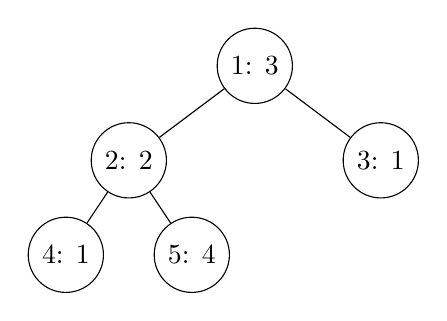
\begin{tikzpicture}[scale=0.8]
    \node[circle, draw] (1) at (2, 3) {1: 3};
    \node[circle, draw] (2) at (0, 1.5) {2: 2};
    \node[circle, draw] (3) at (4, 1.5) {3: 1};
    \node[circle, draw] (4) at (-1, 0) {4: 1};
    \node[circle, draw] (5) at (1, 0) {5: 4};
    
    \draw (1) -- (2);
    \draw (1) -- (3);
    \draw (2) -- (4);
    \draw (2) -- (5);
\end{tikzpicture}
\end{center}

\textbf{后序遍历计算}（先算叶子，再算父节点）：

\textbf{叶子节点}：
\begin{itemize}
    \item $dp[4][0] = 0$，$dp[4][1] = 1$
    \item $dp[5][0] = 0$，$dp[5][1] = 4$
    \item $dp[3][0] = 0$，$dp[3][1] = 1$
\end{itemize}

\textbf{节点 2}（子节点：4, 5）：
\begin{itemize}
    \item $dp[2][0] = \max(0,1) + \max(0,4) = 1 + 4 = 5$
    \item $dp[2][1] = 2 + 0 + 0 = 2$
\end{itemize}

\textbf{节点 1（根）}（子节点：2, 3）：
\begin{itemize}
    \item $dp[1][0] = \max(5,2) + \max(0,1) = 5 + 1 = 6$
    \item $dp[1][1] = 3 + 5 + 0 = 8$
\end{itemize}

\textbf{答案}：$\max(dp[1][0], dp[1][1]) = \max(6, 8) = 8$

\textbf{回溯最优选择}：答案来自 $dp[1][1] = 8$，即\textbf{选节点1}（权值3）。
\begin{itemize}
    \item 选了节点1 $\Rightarrow$ 其子节点2和3\textbf{不能选}（与节点1相邻）。
    \item 对节点2的子树取 $dp[2][0] = 5$（不选节点2时的最优值）：
        \[
        dp[2][0] = \max(dp[4][0], dp[4][1]) + \max(dp[5][0], dp[5][1]) = \max(0,1) + \max(0,4) = 1 + 4 = 5
        \]
        即节点4（权值1）和节点5（权值4）各自独立，\textbf{两者均选}。
    \item 对节点3的子树取 $dp[3][0] = 0$（不选节点3，且节点3为叶子，贡献为0）。
\end{itemize}

因此 $dp[1][1] = w[1] + dp[2][0] + dp[3][0] = 3 + 5 + 0 = 8$。

\textbf{最终答案}：选节点集合 $\{1, 4, 5\}$，权值之和 $= 3 + 1 + 4 = 8$。

\textbf{合法性验证}：节点1与4不相邻（树中路径为1-2-4，无直接边），节点1与5不相邻（路径为1-2-5），节点4与5不相邻（树中无边4-5）。$\checkmark$

\end{blackboard}

%========================================
\subsection{DAG DP：最长路径}
%========================================

\begin{blackboard}[DAG 最长路径问题]

\textbf{问题}：给定有向无环图 (DAG)，边有权重。求从源点到汇点的最长路径。

\textbf{注意}：一般图的最长路径是 NP-hard，但 DAG 上可以用 DP 在 $O(V + E)$ 解决！

\textbf{核心}：DAG 可以拓扑排序，按拓扑序 DP

\textbf{状态}：$dp[v]$ = 从源点到 $v$ 的最长路径长度

\textbf{转移}：
\[
dp[v] = \max_{u \to v} (dp[u] + w(u, v))
\]

\end{blackboard}

\begin{blackboard}[DAG 最长路径例子]

\textbf{输入}：6个节点的 DAG

\begin{center}
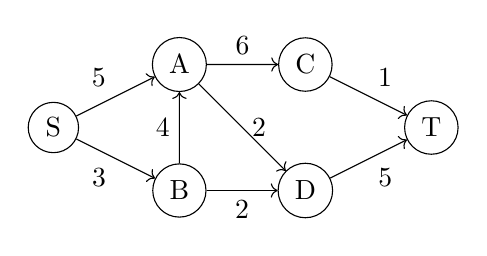
\begin{tikzpicture}[scale=0.8, ->]
    \node[circle, draw] (s) at (0, 1) {S};
    \node[circle, draw] (a) at (2, 2) {A};
    \node[circle, draw] (b) at (2, 0) {B};
    \node[circle, draw] (c) at (4, 2) {C};
    \node[circle, draw] (d) at (4, 0) {D};
    \node[circle, draw] (t) at (6, 1) {T};
    
    \draw (s) -- node[above left] {5} (a);
    \draw (s) -- node[below left] {3} (b);
    \draw (a) -- node[above] {6} (c);
    \draw (a) -- node[right] {2} (d);
    \draw (b) -- node[left] {4} (a);
    \draw (b) -- node[below] {2} (d);
    \draw (c) -- node[above right] {1} (t);
    \draw (d) -- node[below right] {5} (t);
\end{tikzpicture}
\end{center}

\textbf{拓扑排序}：S → B → A → D → C → T

\end{blackboard}

\begin{blackboard}[DAG 最长路径手算]

按拓扑序计算：

\begin{center}
\begin{tabular}{c|l}
节点 & $dp$ 值计算 \\
\hline
S & $dp[S] = 0$（源点） \\
B & $dp[B] = dp[S] + 3 = 3$ \\
A & $dp[A] = \max(dp[S] + 5, dp[B] + 4) = \max(5, 7) = 7$ \\
D & $dp[D] = \max(dp[A] + 2, dp[B] + 2) = \max(9, 5) = 9$ \\
C & $dp[C] = dp[A] + 6 = 13$ \\
T & $dp[T] = \max(dp[C] + 1, dp[D] + 5) = \max(14, 14) = 14$ \\
\end{tabular}
\end{center}

\textbf{答案}：最长路径长度 = 14

\textbf{最长路径}：S → B → A → C → T（$3+4+6+1=14$）

或 S → B → A → D → T（$3+4+2+5=14$）

\end{blackboard}

\begin{blackboard}[DAG DP 的应用]

\textbf{1. 项目调度（关键路径法 CPM）}
\begin{itemize}
    \item 节点 = 任务，边 = 依赖关系
    \item 最长路径 = 项目最短完成时间
    \item 关键路径上的任务不能延迟
\end{itemize}

\textbf{2. 最长递增子序列（LIS）}
\begin{itemize}
    \item 构造 DAG：若 $i < j$ 且 $A[i] < A[j]$，则 $i \to j$
    \item LIS 长度 = DAG 最长路径 + 1
\end{itemize}

\textbf{3. 课程规划}
\begin{itemize}
    \item 节点 = 课程，边 = 先修关系
    \item 最长路径 = 最少需要几个学期
\end{itemize}

\textbf{时间复杂度}：$O(V + E)$（拓扑排序 + 一次遍历）

\end{blackboard}

%========================================
\section{DP 的 GPU 困境与突破}
%========================================

\subsection{为什么 DP 难以并行？}

\begin{blackboard}[DP 的依赖结构]

\textbf{问题}：$dp[i][j]$ 依赖于 $dp[i-1][j]$, $dp[i][j-1]$, $dp[i-1][j-1]$

这意味着：
\begin{itemize}
    \item 不能同时计算 $dp[i][j]$ 和 $dp[i-1][j]$（有依赖）
    \item 不能同时计算 $dp[i][j]$ 和 $dp[i][j-1]$（有依赖）
\end{itemize}

\textbf{传统方法}：逐行或逐列计算，$O(mn)$ 步，无并行！

\textbf{关键洞察}：虽然不能并行计算整行/整列，但可以并行计算\textbf{对角线}！

\end{blackboard}

\subsection{对角线并行（Wavefront 并行）}

\begin{blackboard}[Wavefront 并行的原理]

\textbf{观察}：同一条\textbf{反对角线}上的元素\textbf{互不依赖}！

定义第 $k$ 条对角线：$\{(i, j) : i + j = k\}$

对于 $(i, j)$ 满足 $i + j = k$：
\begin{itemize}
    \item 依赖 $(i-1, j)$：$i-1 + j = k - 1$ ✓ 前一条对角线
    \item 依赖 $(i, j-1)$：$i + j - 1 = k - 1$ ✓ 前一条对角线
    \item 依赖 $(i-1, j-1)$：$i-1+j-1 = k - 2$ ✓ 更早的对角线
\end{itemize}

\textbf{结论}：第 $k$ 条对角线只依赖第 $k-1$ 和 $k-2$ 条，不依赖同一条！

\textbf{并行算法}：
\begin{enumerate}
    \item 按对角线顺序 $k = 0, 1, 2, \ldots, m+n-2$
    \item 每条对角线内，所有元素\textbf{并行计算}
\end{enumerate}

\end{blackboard}

\begin{figure}[ht]
\centering
\begin{tikzpicture}[scale=0.6]
    % 网格
    \draw[step=1, gray!30] (0, 0) grid (7, 8);
    
    % 对角线着色
    \foreach \k/\c in {0/red!20, 1/orange!20, 2/yellow!20, 3/green!20, 4/blue!20, 5/purple!20} {
        \foreach \i in {0,...,7} {
            \pgfmathsetmacro{\j}{\k - \i}
            \pgfmathtruncatemacro{\jint}{\j}
            \ifnum\jint>-1
                \ifnum\jint<8
                    \fill[\c] (\jint, 7-\i) rectangle (\jint+1, 8-\i);
                \fi
            \fi
        }
    }
    
    % 标注
    \node[right] at (8, 7.5) {\small $k=0$};
    \node[right] at (8, 6.5) {\small $k=1$};
    \node[right] at (8, 5.5) {\small $k=2$};
    \node[right] at (8, 4.5) {\small $k=3$};
    
    % 箭头表示计算顺序
    \draw[->, very thick] (0.5, 8.5) -- (7.5, 1.5);
    \node[above] at (4, 8.5) {Wavefront 方向};
    
    % 并行标注
    \draw[<->, thick, gpugreen] (2.2, 4.8) -- (4.8, 2.2);
    \node[gpugreen, right] at (5, 2) {\small 同一对角线并行};
\end{tikzpicture}
\caption{Wavefront 并行：沿对角线方向推进，每条对角线内部并行}
\end{figure}

\begin{complexitybox}[Wavefront 并行的复杂度]

\textbf{总对角线数}：$m + n - 1$

\textbf{最长对角线}：$\min(m, n)$ 个元素

\textbf{并行时间}：$O(m + n)$（假设足够多处理器）

\textbf{加速比}：$\frac{O(mn)}{O(m+n)} = O(\min(m, n))$

\textbf{例}：$m = n = 10000$
\begin{itemize}
    \item 串行：$10^8$ 步
    \item Wavefront 并行：$2 \times 10^4$ 步
    \item 加速比：$5000\times$
\end{itemize}

\end{complexitybox}

\begin{experiment}[编辑距离 GPU 化]
\begin{lstlisting}
import cupy as cp
import numpy as np
import time

def edit_distance_cpu(A, B):
    """CPU版本：标准DP"""
    m, n = len(A), len(B)
    dp = np.zeros((m+1, n+1), dtype=np.int32)
    dp[0, :] = np.arange(n+1)
    dp[:, 0] = np.arange(m+1)
    
    for i in range(1, m+1):
        for j in range(1, n+1):
            if A[i-1] == B[j-1]:
                dp[i, j] = dp[i-1, j-1]
            else:
                dp[i, j] = 1 + min(dp[i-1, j], dp[i, j-1], dp[i-1, j-1])
    return dp[m, n]

def edit_distance_gpu_wavefront(A, B):
    """GPU版本：对角线并行"""
    m, n = len(A), len(B)
    
    # 转换为数值数组
    A_arr = cp.array([ord(c) for c in A], dtype=cp.int32)
    B_arr = cp.array([ord(c) for c in B], dtype=cp.int32)
    
    # DP表格
    dp = cp.zeros((m+1, n+1), dtype=cp.int32)
    dp[0, :] = cp.arange(n+1)
    dp[:, 0] = cp.arange(m+1)
    
    # 对角线并行
    for k in range(2, m + n + 1):
        # 当前对角线的有效范围
        i_start = max(1, k - n)
        i_end = min(m, k - 1)
        
        if i_start > i_end:
            continue
            
        # 构造索引
        i_indices = cp.arange(i_start, i_end + 1)
        j_indices = k - i_indices
        
        # 并行计算这条对角线上的所有元素
        match = (A_arr[i_indices - 1] == B_arr[j_indices - 1]).astype(cp.int32)
        
        candidates = cp.stack([
            dp[i_indices - 1, j_indices] + 1,      # 删除
            dp[i_indices, j_indices - 1] + 1,      # 插入
            dp[i_indices - 1, j_indices - 1] + (1 - match)  # 匹配/替换
        ])
        
        dp[i_indices, j_indices] = cp.min(candidates, axis=0)
    
    return int(dp[m, n])

# 测试
m, n = 5000, 5000
A = ''.join(np.random.choice(list('ACGT'), m))
B = ''.join(np.random.choice(list('ACGT'), n))

# CPU
start = time.time()
dist_cpu = edit_distance_cpu(A, B)
time_cpu = time.time() - start
print(f"CPU: {dist_cpu}, time: {time_cpu:.2f}s")

# GPU
cp.cuda.Stream.null.synchronize()
start = time.time()
dist_gpu = edit_distance_gpu_wavefront(A, B)
cp.cuda.Stream.null.synchronize()
time_gpu = time.time() - start
print(f"GPU: {dist_gpu}, time: {time_gpu:.2f}s")
print(f"Speedup: {time_cpu/time_gpu:.1f}x")
\end{lstlisting}

\textbf{典型结果}（$m = n = 5000$）：
\begin{itemize}
    \item CPU: $\sim$15s
    \item GPU (Wavefront): $\sim$0.3s
    \item 加速比：$\sim 50\times$
\end{itemize}
\end{experiment}

%========================================
\section{贪心算法}
%========================================

\subsection{贪心的核心思想}

\begin{blackboard}[贪心算法的结构]

\textbf{贪心策略}：在每一步选择\textbf{当前看起来最优}的选项。

\textbf{与 DP 的区别}：
\begin{itemize}
    \item DP：考虑所有子问题，选最优组合
    \item 贪心：只做一次选择，不回溯
\end{itemize}

\textbf{贪心正确的条件}：

\begin{enumerate}
    \item \textbf{贪心选择性质}：局部最优选择能导向全局最优
    \item \textbf{最优子结构}：问题的最优解包含子问题的最优解
\end{enumerate}

\textbf{证明技巧：交换论证}

假设存在一个不用贪心选择的最优解，证明可以"交换"成用贪心选择的解，且不变差。

\end{blackboard}

\subsection{例：活动选择问题}

\begin{blackboard}[问题定义]

\textbf{问题}：有 $n$ 个活动，第 $i$ 个活动的时间段是 $[s_i, f_i)$（从 $s_i$ 开始，$f_i$ 结束）。

同一时刻只能参加一个活动。求最多能参加多少个活动。

\textbf{冲突定义}：活动 $i$ 和 $j$ 冲突 $\Leftrightarrow$ $[s_i, f_i) \cap [s_j, f_j) \neq \emptyset$

\textbf{目标}：选择最大的\textbf{互不冲突}的活动子集。

\end{blackboard}

\begin{blackboard}[具体例子]

\textbf{输入}：11 个活动

\begin{center}
\begin{tabular}{c|ccccccccccc}
活动 $i$ & 1 & 2 & 3 & 4 & 5 & 6 & 7 & 8 & 9 & 10 & 11 \\
\hline
开始 $s_i$ & 1 & 3 & 0 & 5 & 3 & 5 & 6 & 8 & 8 & 2 & 12 \\
结束 $f_i$ & 4 & 5 & 6 & 7 & 9 & 9 & 10 & 11 & 12 & 14 & 16 \\
\end{tabular}
\end{center}

\textbf{按结束时间排序后}：

\begin{center}
\begin{tabular}{c|ccccccccccc}
活动 $i$ & 1 & 2 & 3 & 4 & 5 & 6 & 7 & 8 & 9 & 10 & 11 \\
\hline
开始 $s_i$ & 1 & 3 & 0 & 5 & 3 & 5 & 6 & 8 & 8 & 2 & 12 \\
结束 $f_i$ & 4 & 5 & 6 & 7 & 9 & 9 & 10 & 11 & 12 & 14 & 16 \\
\end{tabular}
\end{center}

（这个例子恰好已经按 $f_i$ 排好序了）

\end{blackboard}

\begin{figure}[ht]
\centering
\begin{tikzpicture}[scale=0.45]
    % 时间轴
    \draw[thick, ->] (0, 0) -- (17, 0) node[right] {时间};
    \foreach \t in {0, 2, 4, 6, 8, 10, 12, 14, 16} {
        \draw (\t, -0.2) -- (\t, 0.2);
        \node[below] at (\t, -0.3) {\small \t};
    }
    
    % 活动（按结束时间排列）
    \fill[blue!60] (1, 1) rectangle (4, 1.6);
    \node[left] at (0, 1.3) {\small 1};
    
    \fill[gray!40] (3, 2) rectangle (5, 2.6);
    \node[left] at (0, 2.3) {\small 2};
    
    \fill[gray!40] (0, 3) rectangle (6, 3.6);
    \node[left] at (0, 3.3) {\small 3};
    
    \fill[blue!60] (5, 4) rectangle (7, 4.6);
    \node[left] at (0, 4.3) {\small 4};
    
    \fill[gray!40] (3, 5) rectangle (9, 5.6);
    \node[left] at (0, 5.3) {\small 5};
    
    \fill[gray!40] (5, 6) rectangle (9, 6.6);
    \node[left] at (0, 6.3) {\small 6};
    
    \fill[gray!40] (6, 7) rectangle (10, 7.6);
    \node[left] at (0, 7.3) {\small 7};
    
    \fill[blue!60] (8, 8) rectangle (11, 8.6);
    \node[left] at (0, 8.3) {\small 8};
    
    \fill[gray!40] (8, 9) rectangle (12, 9.6);
    \node[left] at (0, 9.3) {\small 9};
    
    \fill[gray!40] (2, 10) rectangle (14, 10.6);
    \node[left] at (0, 10.3) {\small 10};
    
    \fill[blue!60] (12, 11) rectangle (16, 11.6);
    \node[left] at (0, 11.3) {\small 11};
    
    % 图例
    \fill[blue!60] (18, 10) rectangle (19, 10.6);
    \node[right] at (19.2, 10.3) {\small 选中};
    \fill[gray!40] (18, 9) rectangle (19, 9.6);
    \node[right] at (19.2, 9.3) {\small 未选};
\end{tikzpicture}
\caption{活动选择：贪心选择结束最早的活动，得到 \{1, 4, 8, 11\}，共4个}
\end{figure}

\begin{blackboard}[贪心算法]

\textbf{策略}：每次选择\textbf{结束时间最早}且与已选活动不冲突的活动。

\textbf{算法}：
\begin{algorithmic}[1]
\STATE 将活动按结束时间 $f_i$ 排序
\STATE $S \gets \emptyset$（已选活动集合）
\STATE $last\_finish \gets 0$（上一个选中活动的结束时间）
\FOR{$i = 1$ to $n$}
    \IF{$s_i \geq last\_finish$}
        \STATE $S \gets S \cup \{i\}$
        \STATE $last\_finish \gets f_i$
    \ENDIF
\ENDFOR
\RETURN $S$
\end{algorithmic}

\textbf{时间复杂度}：$O(n \log n)$（排序）+ $O(n)$（遍历）= $O(n \log n)$

\end{blackboard}

\begin{blackboard}[手算过程]

按 $f_i$ 排序后，逐个考虑：

\begin{center}
\begin{tabular}{c|c|c|c|l}
\textbf{考虑} & $s_i$ & $f_i$ & $last\_finish$ & \textbf{决策} \\
\hline
活动1 & 1 & 4 & 0 & $1 \geq 0$ ✓ 选！$last\_finish \gets 4$ \\
活动2 & 3 & 5 & 4 & $3 < 4$ ✗ 冲突，跳过 \\
活动3 & 0 & 6 & 4 & $0 < 4$ ✗ 冲突，跳过 \\
活动4 & 5 & 7 & 4 & $5 \geq 4$ ✓ 选！$last\_finish \gets 7$ \\
活动5 & 3 & 9 & 7 & $3 < 7$ ✗ 冲突，跳过 \\
活动6 & 5 & 9 & 7 & $5 < 7$ ✗ 冲突，跳过 \\
活动7 & 6 & 10 & 7 & $6 < 7$ ✗ 冲突，跳过 \\
活动8 & 8 & 11 & 7 & $8 \geq 7$ ✓ 选！$last\_finish \gets 11$ \\
活动9 & 8 & 12 & 11 & $8 < 11$ ✗ 冲突，跳过 \\
活动10 & 2 & 14 & 11 & $2 < 11$ ✗ 冲突，跳过 \\
活动11 & 12 & 16 & 11 & $12 \geq 11$ ✓ 选！$last\_finish \gets 16$ \\
\end{tabular}
\end{center}

\textbf{结果}：$S = \{1, 4, 8, 11\}$，共 4 个活动。

\end{blackboard}

\subsection{贪心正确性证明：交换论证}

\begin{blackboard}[定理：贪心选择性质]

\textbf{定理}：设 $S$ 是活动集合，$a_1$ 是 $S$ 中结束时间最早的活动。则存在一个包含 $a_1$ 的最优解。

\textbf{证明}（交换论证）：

设 OPT 是任意一个最优解，设 $a_k$ 是 OPT 中\textbf{第一个}（开始最早的）活动。

\textbf{Case 1}：$a_k = a_1$（OPT 的第一个活动就是结束最早的）

已经包含 $a_1$，证毕。 ✓

\textbf{Case 2}：$a_k \neq a_1$

由于 $a_1$ 是所有活动中结束最早的，有 $f_1 \leq f_k$。

构造新解：OPT' $= (\text{OPT} \setminus \{a_k\}) \cup \{a_1\}$

\textbf{验证 OPT' 可行}：

OPT 中 $a_k$ 之后的活动都满足 $s_i \geq f_k$（与 $a_k$ 不冲突）。

由于 $f_1 \leq f_k$，这些活动也满足 $s_i \geq f_k \geq f_1$（与 $a_1$ 不冲突）。

所以 OPT' 中的活动互不冲突。 ✓

\textbf{验证 OPT' 最优}：

$|$OPT'$| = |$OPT$|$（只是替换，数量不变）

所以 OPT' 也是最优解，且包含 $a_1$。 $\square$

\end{blackboard}

\begin{figure}[ht]
\centering
\begin{tikzpicture}[scale=0.5]
    % 上半部分：原始OPT
    \node[left] at (-1, 2) {\textbf{OPT:}};
    \fill[red!60] (2, 1.5) rectangle (6, 2.5);
    \node at (4, 2) {\small $a_k$};
    \fill[blue!40] (7, 1.5) rectangle (10, 2.5);
    \fill[blue!40] (11, 1.5) rectangle (14, 2.5);
    
    % a_1 在下面
    \fill[green!60] (1, 0) rectangle (4, 1);
    \node at (2.5, 0.5) {\small $a_1$};
    \node[right] at (5, 0.5) {\small (结束更早: $f_1 \leq f_k$)};
    
    % 箭头
    \draw[->, thick] (8, 0) -- (8, -1);
    \node[right] at (8.2, -0.5) {\small 交换};
    
    % 下半部分：新的OPT'
    \node[left] at (-1, -2.5) {\textbf{OPT':}};
    \fill[green!60] (1, -3) rectangle (4, -2);
    \node at (2.5, -2.5) {\small $a_1$};
    \fill[blue!40] (7, -3) rectangle (10, -2);
    \fill[blue!40] (11, -3) rectangle (14, -2);
    
    % 说明
    \draw[<->, thick] (4, -3.5) -- (7, -3.5);
    \node[below] at (5.5, -3.7) {\small 仍然不冲突};
\end{tikzpicture}
\caption{交换论证：用 $a_1$ 替换 $a_k$，后续活动仍然不冲突}
\end{figure}

\begin{blackboard}[定理：最优子结构]

\textbf{定理}：设 $a_1$ 是结束最早的活动。若 OPT 是原问题的最优解且 $a_1 \in$ OPT，则 OPT $\setminus \{a_1\}$ 是子问题"$a_1$ 结束后开始的活动"的最优解。

\textbf{子问题定义}：$S' = \{a_i : s_i \geq f_1\}$（所有在 $a_1$ 结束后才开始的活动）

\textbf{证明}（剪切-粘贴）：

设 OPT $\setminus \{a_1\}$ 在子问题 $S'$ 上不是最优。

则存在 $S'$ 的更优解 $B$，满足 $|B| > |$OPT$ \setminus \{a_1\}|$。

构造 $B' = B \cup \{a_1\}$：

\begin{itemize}
    \item $B'$ 可行：$B$ 中的活动都在 $a_1$ 结束后开始，所以与 $a_1$ 不冲突 ✓
    \item $|B'| = |B| + 1 > |$OPT$ \setminus \{a_1\}| + 1 = |$OPT$|$
\end{itemize}

这与 OPT 是最优解矛盾！ $\square$

\end{blackboard}

\begin{blackboard}[完整的归纳证明]

\textbf{定理}：贪心算法得到最优解。

\textbf{证明}（归纳法）：

\textbf{归纳假设}：对于少于 $n$ 个活动的问题，贪心得到最优解。

\textbf{归纳步骤}：考虑 $n$ 个活动的问题。

\begin{enumerate}
    \item 设 $a_1$ 是结束最早的活动。
    \item 由贪心选择性质，存在包含 $a_1$ 的最优解 OPT。
    \item 由最优子结构，OPT $\setminus \{a_1\}$ 是子问题 $S' = \{a_i : s_i \geq f_1\}$ 的最优解。
    \item 子问题 $S'$ 的活动数 $< n$，由归纳假设，贪心在 $S'$ 上得到最优解。
    \item 贪心选择 $a_1$，然后在 $S'$ 上贪心，得到的解 $= \{a_1\} \cup$ (子问题最优解)。
    \item 这与 OPT 大小相同，所以贪心得到最优解。 $\square$
\end{enumerate}

\end{blackboard}

\begin{insight}[为什么选"结束最早"而不是其他策略？]

\textbf{错误策略1}：选开始最早的活动

反例：活动 A=[0, 100)，B=[1, 2)，C=[3, 4)

选 A 只能选 1 个，但选 B, C 能选 2 个。

\textbf{错误策略2}：选持续时间最短的活动

反例：活动 A=[0, 4)，B=[3, 6)，C=[5, 9)

B 最短（3单位），但选 B 只能选 1 个。选 A, C 能选 2 个。

\textbf{错误策略3}：选冲突最少的活动

反例：设有如下 7 个活动：
\begin{itemize}
    \item 中心活动 $M = [3, 7)$，与 $A_1, A_2, A_3$ 均冲突（共 3 次冲突）
    \item 左端活动 $A_1=[1,4)$，$A_2=[2,5)$，$A_3=[3,6)$，各自与 $M$ 冲突，彼此也冲突
    \item 右端活动 $B_1=[5,8)$，$B_2=[6,9)$，$B_3=[7,10)$，各自与 $M$ 冲突，彼此也冲突
\end{itemize}

$M$ 共冲突 6 次，而 $A_i$、$B_j$ 各仅冲突 2--3 次。按"冲突最少"策略，会优先选某个 $A_i$ 或 $B_j$，这将同时排除 $M$ 和另外 $1\sim2$ 个活动；而若直接选 $M$，虽冲突最多，但选完 $M$ 之后左右两侧均无可选活动，只能选 1 个。

直觉上：冲突少的活动往往"挤在一堆"，选了它反而阻塞了其他互相兼容的活动；选结束最早的活动才能保证给后续留下最大余地。

\textbf{为什么"结束最早"是对的？}

直觉：尽早结束 $\Rightarrow$ 给后面留更多空间 $\Rightarrow$ 能选更多活动

这个直觉被交换论证严格证明了。
\end{insight}

\subsection{更多贪心经典例子}

\subsubsection{例：分数背包}

\begin{blackboard}[分数背包 vs 0-1背包]

\textbf{0-1背包}：物品要么完整拿，要么不拿（DP解决）

\textbf{分数背包}：物品可以\textbf{拿一部分}（贪心解决！）

\textbf{问题}：$n$ 个物品，第 $i$ 个重量 $w_i$，价值 $v_i$。背包容量 $W$。

可以拿物品的任意比例 $0 \leq x_i \leq 1$。

最大化 $\sum_i x_i \cdot v_i$，约束 $\sum_i x_i \cdot w_i \leq W$。

\textbf{贪心策略}：按\textbf{单位价值} $v_i / w_i$ 从大到小排序，依次尽量多拿。

\end{blackboard}

\begin{blackboard}[分数背包例子]

\textbf{输入}：背包容量 $W = 50$

\begin{center}
\begin{tabular}{c|ccc}
物品 & 重量 $w_i$ & 价值 $v_i$ & 单位价值 $v_i/w_i$ \\
\hline
A & 10 & 60 & 6 \\
B & 20 & 100 & 5 \\
C & 30 & 120 & 4 \\
\end{tabular}
\end{center}

\textbf{按单位价值排序}：A (6) > B (5) > C (4)

\textbf{贪心过程}：
\begin{itemize}
    \item 拿 A：全部拿，用掉容量 10，价值 60，剩余容量 40
    \item 拿 B：全部拿，用掉容量 20，价值 100，剩余容量 20
    \item 拿 C：只能拿 20/30 = 2/3，价值 $120 \times \frac{2}{3} = 80$
\end{itemize}

\textbf{总价值}：$60 + 100 + 80 = 240$

\end{blackboard}

\begin{blackboard}[分数背包贪心正确性证明]

\textbf{定理}：按单位价值排序的贪心策略是最优的。

\textbf{证明}（交换论证）：

设物品已按 $v_1/w_1 \geq v_2/w_2 \geq \cdots \geq v_n/w_n$ 排序。

设 OPT 是最优解，$x_i^*$ 是物品 $i$ 的取用比例。

设贪心解为 $x_i^G$。

假设 OPT $\neq$ 贪心解，找第一个不同的位置 $k$：$x_k^* < x_k^G$。

由于贪心尽量多拿前面的物品，必存在 $j > k$ 使得 $x_j^* > x_j^G$。

\textbf{交换}：增加 $x_k$，减少 $x_j$，保持总重量不变。

设增量为 $\Delta$，则价值变化为：
\[
\Delta \cdot v_k / w_k - \Delta \cdot v_j / w_j = \Delta \left( \frac{v_k}{w_k} - \frac{v_j}{w_j} \right) \geq 0
\]

因为 $k < j$ 意味着 $v_k/w_k \geq v_j/w_j$。

所以交换后价值不减，OPT 可以逐步变成贪心解。 $\square$

\end{blackboard}

\subsubsection{例：跳跃游戏}

\begin{blackboard}[跳跃游戏（LeetCode 55）]

\textbf{问题}：数组 $A[0..n-1]$，$A[i]$ 表示从位置 $i$ 最多能跳 $A[i]$ 步。

从位置 0 出发，能否到达位置 $n-1$？

\textbf{例1}：$A = [2, 3, 1, 1, 4]$ → \textbf{能}（0→1→4 或 0→2→3→4）

\textbf{例2}：$A = [3, 2, 1, 0, 4]$ → \textbf{不能}（卡在位置3）

\textbf{贪心策略}：维护当前能到达的最远位置 $maxReach$

\end{blackboard}

\begin{blackboard}[跳跃游戏贪心算法]

\begin{algorithmic}[1]
\STATE $maxReach \gets 0$
\FOR{$i = 0$ to $n-1$}
    \IF{$i > maxReach$}
        \RETURN False \COMMENT{当前位置不可达}
    \ENDIF
    \STATE $maxReach \gets \max(maxReach, i + A[i])$
    \IF{$maxReach \geq n-1$}
        \RETURN True
    \ENDIF
\ENDFOR
\RETURN True
\end{algorithmic}

\textbf{时间复杂度}：$O(n)$

\end{blackboard}

\begin{blackboard}[跳跃游戏手算]

\textbf{输入}：$A = [2, 3, 1, 1, 4]$

\begin{center}
\begin{tabular}{c|ccccc}
$i$ & 0 & 1 & 2 & 3 & 4 \\
\hline
$A[i]$ & 2 & 3 & 1 & 1 & 4 \\
$maxReach$ & 2 & 4 & 4 & 4 & -- \\
\end{tabular}
\end{center}

\textbf{过程}：
\begin{itemize}
    \item $i=0$：$0 \leq maxReach=0$ ✓，更新 $maxReach = \max(0, 0+2) = 2$
    \item $i=1$：$1 \leq 2$ ✓，更新 $maxReach = \max(2, 1+3) = 4 \geq 4$，\textbf{返回 True}
\end{itemize}

\textbf{输入}：$A = [3, 2, 1, 0, 4]$

\begin{center}
\begin{tabular}{c|ccccc}
$i$ & 0 & 1 & 2 & 3 & 4 \\
\hline
$A[i]$ & 3 & 2 & 1 & 0 & 4 \\
$maxReach$ & 3 & 3 & 3 & 3 & -- \\
\end{tabular}
\end{center}

\textbf{过程}：
\begin{itemize}
    \item $i=0$：$maxReach = 3$
    \item $i=1$：$maxReach = \max(3, 3) = 3$
    \item $i=2$：$maxReach = \max(3, 3) = 3$
    \item $i=3$：$maxReach = \max(3, 3) = 3$
    \item $i=4$：$4 > maxReach = 3$，\textbf{返回 False}
\end{itemize}

\end{blackboard}

\subsubsection{例：加油站问题}

\begin{blackboard}[加油站问题（LeetCode 134）]

\textbf{问题}：环形路线上有 $n$ 个加油站。第 $i$ 站有汽油 $gas[i]$，到下一站需要 $cost[i]$。

从某站出发（油箱初始为空），能否绕一圈回到起点？若能，返回起点编号。

\textbf{例}：$gas = [1, 2, 3, 4, 5]$，$cost = [3, 4, 5, 1, 2]$

净收益：$[-2, -2, -2, 3, 3]$

从站3出发：$4-1=3 \to 3+5-2=6 \to 6+1-3=4 \to 4+2-4=2 \to 2+3-5=0$ ✓

\textbf{答案}：站3

\end{blackboard}

\begin{blackboard}[加油站贪心算法]

\textbf{关键观察}：

1. 若 $\sum gas[i] < \sum cost[i]$，则无解（总油量不够）

2. 若从站 $i$ 出发，在站 $j$ 油量变负，则 $i$ 到 $j$ 之间任何站都不能作为起点

\textbf{贪心策略}：
\begin{algorithmic}[1]
\STATE $totalTank \gets 0$, $currTank \gets 0$, $start \gets 0$
\FOR{$i = 0$ to $n-1$}
    \STATE $totalTank \gets totalTank + gas[i] - cost[i]$
    \STATE $currTank \gets currTank + gas[i] - cost[i]$
    \IF{$currTank < 0$}
        \STATE $start \gets i + 1$ \COMMENT{从下一站重新开始}
        \STATE $currTank \gets 0$
    \ENDIF
\ENDFOR
\IF{$totalTank \geq 0$}
    \RETURN $start$
\ELSE
    \RETURN $-1$
\ENDIF
\end{algorithmic}

\end{blackboard}

\begin{blackboard}[加油站手算]

\textbf{输入}：$gas = [1, 2, 3, 4, 5]$，$cost = [3, 4, 5, 1, 2]$

\begin{center}
\begin{tabular}{c|ccccc}
$i$ & 0 & 1 & 2 & 3 & 4 \\
\hline
$gas[i] - cost[i]$ & -2 & -2 & -2 & 3 & 3 \\
$currTank$ & -2→0 & -2→0 & -2→0 & 3 & 6 \\
$start$ & 1 & 2 & 3 & 3 & 3 \\
\end{tabular}
\end{center}

$totalTank = -2-2-2+3+3 = 0 \geq 0$

\textbf{答案}：$start = 3$

\textbf{正确性}：若从0,1,2出发都会在某处油量变负，它们之间任何站也不行（因为到达那些站时油量$\geq 0$，从那里出发只会更差），所以必须从3开始。

\end{blackboard}

\subsubsection{例：最小化最大延迟（配对型交换）}

\begin{blackboard}[最小化最大延迟问题]

\textbf{问题}：$n$ 个任务，第 $i$ 个任务需要处理时间 $t_i$，截止时间 $d_i$。

单机串行处理，最小化\textbf{最大延迟} $\max_i (f_i - d_i)$，其中 $f_i$ 是任务 $i$ 的完成时间。

\textbf{例}：3个任务

\begin{center}
\begin{tabular}{c|ccc}
任务 & 1 & 2 & 3 \\
\hline
处理时间 $t_i$ & 3 & 2 & 1 \\
截止时间 $d_i$ & 6 & 8 & 9 \\
\end{tabular}
\end{center}

\textbf{贪心策略}：按截止时间 $d_i$ 从早到晚排序（EDF: Earliest Deadline First）

\end{blackboard}

\begin{blackboard}[最小化最大延迟手算]

\textbf{按 $d_i$ 排序}：任务顺序 1 → 2 → 3

\textbf{计算完成时间和延迟}：

\begin{center}
\begin{tabular}{c|cccc}
任务 & 开始 & 完成 $f_i$ & 截止 $d_i$ & 延迟 $f_i - d_i$ \\
\hline
1 & 0 & 3 & 6 & -3 \\
2 & 3 & 5 & 8 & -3 \\
3 & 5 & 6 & 9 & -3 \\
\end{tabular}
\end{center}

\textbf{最大延迟}：$\max(-3, -3, -3) = -3$（所有任务都提前完成）

\textbf{如果用其他顺序}（比如 3 → 2 → 1）：

\begin{center}
\begin{tabular}{c|cccc}
任务 & 开始 & 完成 $f_i$ & 截止 $d_i$ & 延迟 $f_i - d_i$ \\
\hline
3 & 0 & 1 & 9 & -8 \\
2 & 1 & 3 & 8 & -5 \\
1 & 3 & 6 & 6 & 0 \\
\end{tabular}
\end{center}

最大延迟 = 0，比 EDF 的 -3 更差！

\end{blackboard}

\begin{blackboard}[EDF 正确性证明（配对型交换）]

\textbf{定理}：EDF（按截止时间排序）最小化最大延迟。

\textbf{证明}（交换论证）：

设 OPT 是最优调度。若 OPT 不是 EDF 顺序，则存在\textbf{逆序对}：

相邻任务 $i, j$ 满足 $i$ 在 $j$ 前面执行，但 $d_i > d_j$。

\textbf{交换动作}：交换 $i$ 和 $j$ 的执行顺序。

\textbf{分析交换后的延迟变化}：

设交换前 $i$ 从时刻 $s$ 开始。

\begin{center}
\begin{tabular}{c|cc}
 & 交换前 & 交换后 \\
\hline
任务 $j$ 完成时间 & $s + t_i + t_j$ & $s + t_j$ \\
任务 $i$ 完成时间 & $s + t_i$ & $s + t_j + t_i$ \\
\end{tabular}
\end{center}

\textbf{关键观察}：

交换前 $j$ 的延迟：$(s + t_i + t_j) - d_j$

交换后 $i$ 的延迟：$(s + t_j + t_i) - d_i$

由于 $d_i > d_j$，有：
\[
(s + t_i + t_j) - d_i < (s + t_i + t_j) - d_j
\]

所以交换后 $i$ 的新延迟 $<$ 交换前 $j$ 的延迟。

而 $j$ 的新延迟 $(s + t_j) - d_j < (s + t_i + t_j) - d_j$（更早完成）。

\textbf{结论}：交换后最大延迟不增。重复消除逆序对，最终得到 EDF。$\square$

\end{blackboard}

\begin{figure}[ht]
\centering
\begin{tikzpicture}[scale=0.6]
    % 交换前
    \node[left] at (-1, 1.5) {\textbf{交换前}:};
    \fill[red!40] (0, 1) rectangle (3, 2);
    \node at (1.5, 1.5) {$i$};
    \fill[blue!40] (3, 1) rectangle (5, 2);
    \node at (4, 1.5) {$j$};
    
    % 截止时间标记
    \draw[dashed, red] (4.5, 0.8) -- (4.5, 2.2);
    \node[red, below] at (4.5, 0.7) {\small $d_i$};
    \draw[dashed, blue] (3.5, 0.8) -- (3.5, 2.2);
    \node[blue, below] at (3.5, 0.7) {\small $d_j$};
    
    % 箭头
    \draw[->, thick] (6, 1.5) -- (8, 1.5);
    \node[above] at (7, 1.5) {\small 交换};
    
    % 交换后
    \node[left] at (8, 1.5) {};
    \fill[blue!40] (9, 1) rectangle (11, 2);
    \node at (10, 1.5) {$j$};
    \fill[red!40] (11, 1) rectangle (14, 2);
    \node at (12.5, 1.5) {$i$};
    
    % 截止时间标记
    \draw[dashed, red] (13.5, 0.8) -- (13.5, 2.2);
    \node[red, below] at (13.5, 0.7) {\small $d_i$};
    \draw[dashed, blue] (12.5, 0.8) -- (12.5, 2.2);
    \node[blue, below] at (12.5, 0.7) {\small $d_j$};
    
    % 说明
    \node at (7, -0.5) {$d_j < d_i$，交换后 $j$ 提前完成，$i$ 的新延迟 $\leq j$ 的旧延迟};
\end{tikzpicture}
\caption{配对型交换：交换相邻逆序对，最大延迟不增}
\end{figure}

\subsubsection{例：霍夫曼编码}

\begin{blackboard}[霍夫曼编码问题]

\textbf{问题}：给定字符集及其频率，设计\textbf{前缀编码}使得平均编码长度最小。

\textbf{前缀编码}：任何字符的编码都不是另一个字符编码的前缀。

\textbf{例}：字符频率

\begin{center}
\begin{tabular}{c|cccccc}
字符 & a & b & c & d & e & f \\
\hline
频率 & 45 & 13 & 12 & 16 & 9 & 5 \\
\end{tabular}
\end{center}

\textbf{目标}：最小化 $\sum_i f_i \cdot l_i$（频率 × 编码长度）

\end{blackboard}

\begin{blackboard}[霍夫曼算法]

\textbf{贪心策略}：
\begin{enumerate}
    \item 将每个字符作为单节点树，权重 = 频率
    \item 重复：取权重最小的两棵树，合并成一棵新树，权重 = 两者之和
    \item 直到只剩一棵树
\end{enumerate}

\textbf{编码}：从根到叶子，左边记 0，右边记 1

\end{blackboard}

\begin{blackboard}[霍夫曼编码手算]

\textbf{输入}：a:45, b:13, c:12, d:16, e:9, f:5

\textbf{Step 1}：合并最小的 f(5) 和 e(9) → (f,e):14

剩余：a:45, d:16, (f,e):14, b:13, c:12

\textbf{Step 2}：合并 c(12) 和 b(13) → (c,b):25

剩余：a:45, (c,b):25, d:16, (f,e):14

\textbf{Step 3}：合并 (f,e)(14) 和 d(16) → ((f,e),d):30

剩余：a:45, ((f,e),d):30, (c,b):25

\textbf{Step 4}：合并 (c,b)(25) 和 ((f,e),d)(30) → 55

剩余：a:45, 55

\textbf{Step 5}：合并 a(45) 和 55 → 100（根）

\end{blackboard}

\begin{figure}[ht]
\centering
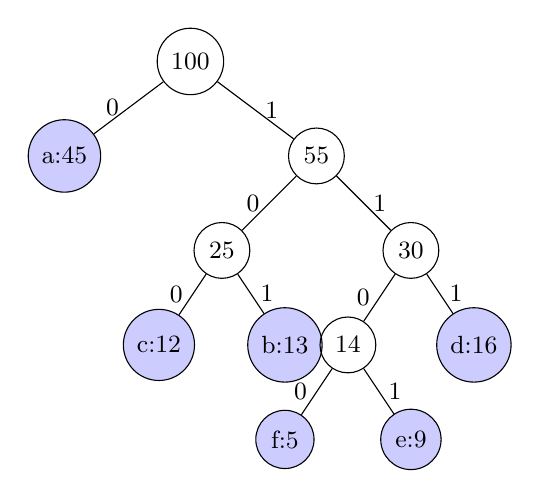
\begin{tikzpicture}[scale=0.8, every node/.style={font=\small}]
    % 根
    \node[circle, draw] (root) at (0, 0) {100};
    
    % 第一层
    \node[circle, draw, fill=blue!20] (a) at (-2, -1.5) {a:45};
    \node[circle, draw] (n55) at (2, -1.5) {55};
    
    \draw (root) -- node[left] {0} (a);
    \draw (root) -- node[right] {1} (n55);
    
    % 第二层
    \node[circle, draw] (cb) at (0.5, -3) {25};
    \node[circle, draw] (fed) at (3.5, -3) {30};
    
    \draw (n55) -- node[left] {0} (cb);
    \draw (n55) -- node[right] {1} (fed);
    
    % 第三层
    \node[circle, draw, fill=blue!20] (c) at (-0.5, -4.5) {c:12};
    \node[circle, draw, fill=blue!20] (b) at (1.5, -4.5) {b:13};
    \node[circle, draw] (fe) at (2.5, -4.5) {14};
    \node[circle, draw, fill=blue!20] (d) at (4.5, -4.5) {d:16};
    
    \draw (cb) -- node[left] {0} (c);
    \draw (cb) -- node[right] {1} (b);
    \draw (fed) -- node[left] {0} (fe);
    \draw (fed) -- node[right] {1} (d);
    
    % 第四层
    \node[circle, draw, fill=blue!20] (f) at (1.5, -6) {f:5};
    \node[circle, draw, fill=blue!20] (e) at (3.5, -6) {e:9};
    
    \draw (fe) -- node[left] {0} (f);
    \draw (fe) -- node[right] {1} (e);
\end{tikzpicture}
\caption{霍夫曼树：高频字符(a)靠近根，低频字符(f,e)远离根}
\end{figure}

\begin{blackboard}[霍夫曼编码结果]

\begin{center}
\begin{tabular}{c|ccc}
字符 & 频率 & 编码 & 长度 \\
\hline
a & 45 & 0 & 1 \\
c & 12 & 100 & 3 \\
b & 13 & 101 & 3 \\
f & 5 & 1100 & 4 \\
e & 9 & 1101 & 4 \\
d & 16 & 111 & 3 \\
\end{tabular}
\end{center}

\textbf{平均编码长度}：
\[
\frac{45 \times 1 + 12 \times 3 + 13 \times 3 + 5 \times 4 + 9 \times 4 + 16 \times 3}{100} = \frac{224}{100} = 2.24
\]

\textbf{对比定长编码}：6个字符需要 $\lceil \log_2 6 \rceil = 3$ 位

霍夫曼节省了 $\frac{3 - 2.24}{3} \approx 25\%$

\end{blackboard}

\subsubsection{例：最小生成树（切割型交换）}

\begin{blackboard}[最小生成树问题]

\textbf{问题}：给定连通无向图 $G = (V, E)$，边权 $w: E \to \mathbb{R}^+$。

求边权和最小的生成树（连接所有顶点的无环子图）。

\textbf{两个经典贪心算法}：

\textbf{Kruskal}：按边权从小到大排序，依次加入不形成环的边

\textbf{Prim}：从任意顶点出发，每次加入连接树与非树顶点的最小边

\end{blackboard}

\begin{blackboard}[Kruskal 算法例子]

\textbf{输入}：6个顶点，9条边

\begin{center}
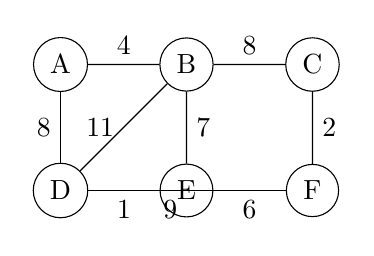
\begin{tikzpicture}[scale=0.8]
    \node[circle, draw] (a) at (0, 2) {A};
    \node[circle, draw] (b) at (2, 2) {B};
    \node[circle, draw] (c) at (4, 2) {C};
    \node[circle, draw] (d) at (0, 0) {D};
    \node[circle, draw] (e) at (2, 0) {E};
    \node[circle, draw] (f) at (4, 0) {F};
    
    \draw (a) -- node[above] {4} (b);
    \draw (b) -- node[above] {8} (c);
    \draw (a) -- node[left] {8} (d);
    \draw (b) -- node[left] {11} (d);
    \draw (b) -- node[right] {7} (e);
    \draw (c) -- node[right] {2} (f);
    \draw (d) -- node[below] {1} (e);
    \draw (e) -- node[below] {6} (f);
    \draw (d) -- node[below left] {9} (f);
\end{tikzpicture}
\end{center}

\textbf{边按权重排序}：(D,E):1, (C,F):2, (A,B):4, (E,F):6, (B,E):7, (A,D):8, (B,C):8, (D,F):9, (B,D):11

\end{blackboard}

\begin{blackboard}[Kruskal 手算过程]

\begin{center}
\begin{tabular}{c|c|c|l}
\textbf{步骤} & \textbf{边} & \textbf{权重} & \textbf{决策} \\
\hline
1 & (D,E) & 1 & 加入（D和E在不同组件）\\
2 & (C,F) & 2 & 加入（C和F在不同组件）\\
3 & (A,B) & 4 & 加入（A和B在不同组件）\\
4 & (E,F) & 6 & 加入（连接\{D,E\}和\{C,F\}）\\
5 & (B,E) & 7 & 加入（连接\{A,B\}和\{C,D,E,F\}）\\
6 & (A,D) & 8 & \textcolor{red}{跳过}（A和D已连通）\\
7 & (B,C) & 8 & \textcolor{red}{跳过}（B和C已连通）\\
\end{tabular}
\end{center}

\textbf{MST 边集}：\{(D,E), (C,F), (A,B), (E,F), (B,E)\}

\textbf{总权重}：$1 + 2 + 4 + 6 + 7 = 20$

\end{blackboard}

\begin{figure}[ht]
\centering
\begin{tikzpicture}[scale=0.8]
    \node[circle, draw, fill=blue!20] (a) at (0, 2) {A};
    \node[circle, draw, fill=blue!20] (b) at (2, 2) {B};
    \node[circle, draw, fill=blue!20] (c) at (4, 2) {C};
    \node[circle, draw, fill=blue!20] (d) at (0, 0) {D};
    \node[circle, draw, fill=blue!20] (e) at (2, 0) {E};
    \node[circle, draw, fill=blue!20] (f) at (4, 0) {F};
    
    % MST边（粗线）
    \draw[very thick, red] (a) -- node[above] {4} (b);
    \draw[very thick, red] (b) -- node[right] {7} (e);
    \draw[very thick, red] (c) -- node[right] {2} (f);
    \draw[very thick, red] (d) -- node[below] {1} (e);
    \draw[very thick, red] (e) -- node[below] {6} (f);
    
    % 非MST边（虚线）
    \draw[dashed, gray] (b) -- node[above] {8} (c);
    \draw[dashed, gray] (a) -- node[left] {8} (d);
    \draw[dashed, gray] (b) -- node[left] {11} (d);
    \draw[dashed, gray] (d) -- node[below left] {9} (f);
    
    \node at (2, -1.5) {MST 总权重 = 20};
\end{tikzpicture}
\caption{Kruskal 算法得到的最小生成树（红色粗边）}
\end{figure}

\begin{blackboard}[Cut Property（割性质）]

\textbf{定义}：图 $G$ 的一个\textbf{割} $(S, V \setminus S)$ 是顶点集的一个划分。

\textbf{跨割边}：一端在 $S$，一端在 $V \setminus S$ 的边。

\textbf{Cut Property}：设 $(S, V \setminus S)$ 是任意割，$e$ 是跨割边中权重最小的（唯一最小）。则 $e$ 属于某棵 MST。

\end{blackboard}

\begin{blackboard}[Cut Property 证明（切割型交换）]

\textbf{证明}：

设 $T^*$ 是任意 MST。

\textbf{Case 1}：$e \in T^*$，证毕。

\textbf{Case 2}：$e \notin T^*$。

将 $e$ 加入 $T^*$ 会形成唯一的环 $C$。

环 $C$ 必然还包含另一条跨割边 $e'$（因为 $e$ 跨割，环必须"回来"）。

由假设，$w(e) < w(e')$。

\textbf{交换}：$T' = T^* \cup \{e\} \setminus \{e'\}$

\textbf{验证}：
\begin{itemize}
    \item $T'$ 仍连通：删 $e'$ 断开的两部分被 $e$ 重新连接
    \item $T'$ 无环：删除了环 $C$ 中的一条边
    \item $w(T') = w(T^*) - w(e') + w(e) < w(T^*)$
\end{itemize}

与 $T^*$ 是 MST 矛盾！所以 Case 2 不可能。 $\square$

\end{blackboard}

\begin{figure}[ht]
\centering
\begin{tikzpicture}[scale=0.7]
    % 割
    \draw[thick, dashed, orange] (3, -1) -- (3, 4);
    \node[orange] at (3, 4.3) {割};
    
    % S侧
    \node[circle, draw, fill=blue!20] (a) at (1, 3) {A};
    \node[circle, draw, fill=blue!20] (b) at (1, 1) {B};
    \node at (1, -0.5) {$S$};
    
    % V\S侧
    \node[circle, draw, fill=green!20] (c) at (5, 3) {C};
    \node[circle, draw, fill=green!20] (d) at (5, 1) {D};
    \node at (5, -0.5) {$V \setminus S$};
    
    % MST边
    \draw[very thick] (a) -- (b);
    \draw[very thick] (c) -- (d);
    \draw[very thick, red, dashed] (b) -- node[below] {$e'$: 重} (c);
    
    % 最小跨割边
    \draw[very thick, green!60!black] (a) -- node[above] {$e$: 轻} (c);
    
    % 环
    \draw[->, thick, blue] (6, 2) arc (0:180:0.5);
    \node[blue, right] at (6.5, 2) {加入 $e$ 形成环};
\end{tikzpicture}
\caption{Cut Property：最小跨割边 $e$ 必在 MST 中，否则可以替换 $e'$}
\end{figure}

\begin{blackboard}[Kruskal 正确性（基于 Cut Property）]

\textbf{为什么 Kruskal 正确？}

当 Kruskal 选择边 $e = (u, v)$ 时：

\begin{itemize}
    \item $u$ 和 $v$ 在不同的连通分量（否则会形成环）
    \item 设 $u$ 所在分量为 $S$，则 $(S, V \setminus S)$ 是一个割
    \item $e$ 是\textbf{目前未考虑的边中}权重最小的跨割边
    \item 由 Cut Property，$e$ 属于某棵 MST
\end{itemize}

\textbf{归纳}：每一步选的边都在某棵 MST 中，最终得到 MST。

\end{blackboard}

\begin{keypoint}[贪心交换论证的四种类型总结]

\textbf{A. 排序型}（活动选择、区间调度）
\begin{itemize}
    \item 交换对象：第一个被选的元素
    \item 关键：贪心选的"结束更早/更小" $\Rightarrow$ 不减少后续空间
\end{itemize}

\textbf{B. 配对型}（最小化最大延迟、任务调度）
\begin{itemize}
    \item 交换对象：相邻逆序对
    \item 关键：消除逆序后目标函数不增
\end{itemize}

\textbf{C. 切割型}（MST 的 Cut Property）
\begin{itemize}
    \item 交换对象：跨割的一条"重边"
    \item 关键：换成最轻边后仍是生成树，且更优
\end{itemize}

\textbf{D. 资源分配型}（分数背包、霍夫曼编码）
\begin{itemize}
    \item 交换对象：资源份额或编码深度
    \item 关键：把"更该优先的"往前挪，目标单调改进
\end{itemize}

\end{keypoint}

\subsection{贪心为什么难并行？}

\begin{gpubox}[贪心的顺序依赖]

\textbf{问题}：贪心的每一步都依赖前一步的结果！

活动选择的贪心过程：
\begin{enumerate}
    \item 选结束最早的活动 $a_1$
    \item 在 $a_1$ 结束后开始的活动中，选结束最早的 $a_2$
    \item 在 $a_2$ 结束后开始的活动中，选结束最早的 $a_3$
    \item $\cdots$
\end{enumerate}

每一步的\textbf{候选集}取决于前一步的选择，无法并行！

\textbf{并行化思路}：
\begin{itemize}
    \item 预处理可以并行（如排序）
    \item 但核心的贪心选择过程很难并行
    \item 有时可以用"并行暴力"替代贪心
\end{itemize}

\end{gpubox}

%========================================
\section{暴力的逆袭：当并行改变一切}
%========================================

\subsection{核心思想}

\begin{insight}[复杂度的重新审视]

传统算法分析假设\textbf{顺序执行}：$O(n^2)$ 比 $O(n)$ 慢。

但在GPU上，这个关系可能\textbf{颠倒}！

\textbf{关键公式}：
\[
\text{实际时间} = \frac{\text{总工作量}}{\text{并行度}}
\]

\begin{itemize}
    \item 聪明算法 $O(n)$，但只能串行 $\Rightarrow$ 时间 $O(n)$
    \item 笨算法 $O(n^2)$，但完全并行 $\Rightarrow$ 时间 $O(n^2 / p)$
\end{itemize}

当 $p > n$ 时，$O(n^2/p) < O(n)$，暴力更快！

\end{insight}




\begin{keypoint}[什么时候暴力能赢]

\textbf{暴力更快的条件}：
\begin{enumerate}
    \item 问题规模较小（暴力的总工作量不太大）
    \item 暴力算法完全并行（每个实例独立）
    \item 聪明算法有串行依赖（无法充分利用GPU）
    \item GPU有足够多的核心（并行度 > 问题规模）
\end{enumerate}

\textbf{实际应用}：
\begin{itemize}
    \item 小规模子问题：用GPU暴力
    \item 大规模问题：用传统算法或混合策略
\end{itemize}

\end{keypoint}

%========================================
\section{总结与实验}
%========================================

\begin{keypoint}[本周要点]

\begin{enumerate}
    \item \textbf{分治}：子问题独立 $\Rightarrow$ 天然并行
    \begin{itemize}
        \item Merge Sort：层级并行
        \item FFT：蝴蝶操作并行
    \end{itemize}
    
    \item \textbf{动态规划}：有依赖但可以找并行结构
    \begin{itemize}
        \item Wavefront 并行：沿对角线推进
        \item 加速比可达 $O(\min(m,n))$
    \end{itemize}
    
    \item \textbf{贪心}：顺序依赖最强，最难并行
    \begin{itemize}
        \item 预处理可以并行
        \item 核心贪心选择通常串行
    \end{itemize}
    
    \item \textbf{暴力的逆袭}：当并行度足够高
    \begin{itemize}
        \item $O(n^2)$ 并行可能快于 $O(n)$ 串行
        \item 关键是找到临界点
    \end{itemize}
\end{enumerate}

\end{keypoint}



\appendix
\section{附录：CUDA Kernel 示例}

\begin{lstlisting}[language=C, caption={并行合并的 CUDA Kernel}]
__global__ void parallel_merge_kernel(
    float* A, float* B, float* C,
    int m, int n
) {
    int tid = blockIdx.x * blockDim.x + threadIdx.x;
    int total = m + n;
    
    if (tid >= total) return;
    
    // 二分搜索找到正确的分割点
    int low = max(0, tid - n);
    int high = min(tid, m);
    
    while (low < high) {
        int mid = (low + high) / 2;
        int j = tid - mid;
        
        if (j > 0 && mid < m && B[j-1] > A[mid]) {
            low = mid + 1;
        } else {
            high = mid;
        }
    }
    
    int i = low;
    int j = tid - i;
    
    // 确定C[tid]的值
    if (i >= m) {
        C[tid] = B[j];
    } else if (j >= n) {
        C[tid] = A[i];
    } else {
        C[tid] = (A[i] <= B[j]) ? A[i] : B[j];
    }
}
\end{lstlisting}

\end{document}